\documentclass[11pt,a4paper]{article}
\usepackage{fontspec}
\setmainfont{TeX Gyre Pagella}
\newfontfamily\headfont{Inter}[UprightFont=*-ExtraBold,BoldFont=*-ExtraBold,Extension=.otf,Path=/usr/share/fonts/opentype/inter/]
\usepackage[a4paper,margin=2.3cm]{geometry}
\usepackage{amsmath}
\usepackage{graphicx,booktabs,float,caption,array,xcolor,longtable,threeparttable}
\usepackage{xurl}
\usepackage[hidelinks]{hyperref}
\usepackage{titlesec}
\usepackage[round]{natbib}
\usepackage{setspace}
\setstretch{1.05}
\renewcommand{\topfraction}{0.9}
\renewcommand{\bottomfraction}{0.8}
\renewcommand{\textfraction}{0.1}
\renewcommand{\floatpagefraction}{0.75}
\setlength{\parindent}{0pt}
\setlength{\parskip}{0.55em}
\titleformat{\section}{\headfont\Large}{\thesection}{0.8em}{}
\titleformat{\subsection}{\headfont\large}{\thesubsection}{0.8em}{}
\captionsetup{font=small,labelfont=bf}
\urlstyle{same}
\hypersetup{pdftitle={Gladstone Road or Disraeli Street?},pdfauthor={Dr Tristan Hotham}}

\begin{document}
\begin{center}
{\Large\bfseries Gladstone Road or Disraeli Street? Partisan Commemoration in the Street Names of Victorian Britain\par}
\vspace{1.2em}
{\large Dr Tristan Hotham\par}
\vspace{0.3em}
{\small Independent researcher\\
ORCID: 0000-0003-4931-9349\\
DOI: https://doi.org/10.5281/zenodo.24092657\par}
\vspace{0.8em}
2026
\end{center}

\begin{quote}
\small
\begin{center}\textbf{Abstract}\end{center}
Victorian builders, landowners and councils named thousands of streets after statesmen, but did the names they chose follow local politics? I build a national table of commemorative street names from OpenStreetMap (15,593 streets), with a name table that separates unambiguous party commemorations (Gladstone, Cobden, John Bright and Palmerston; Beaconsfield and Disraeli) from names that are mostly places or surnames, using a pre-set co-location test. I link 160 British towns to the general election results of the constituencies named after them, 1868 to 1900. Liberal names outnumber Conservative ones about 3.4 to 1 almost everywhere. In the main model, fixed in a written analysis plan before any outcome model was run (a street-level linear probability model with region fixed effects and errors clustered by town), each 10 points of Liberal vote is associated with a 5.9 point higher Liberal share of a town's party street names (95\% CI 0.4 to 11.4; 610 streets). The association survives randomisation inference, leaving out any region and most measurement choices, and is absent with the vote of 1945 to 1970. It is weak, however: it is not significant in an unweighted town-level model, in the boroughs of 1868 alone, in either half of the period, or with the share of seats won, and exploratory checks show it is carried by Beaconsfield names. Battle streets roughly date the party names to the late Victorian decades. The design is correlational: street names record partisan memory, but only faintly the politics of the town around them.

\textbf{Keywords:} street names; commemoration; political memory; Gladstone; Disraeli; Victorian elections; electoral geography; OpenStreetMap
\end{quote}

\section{Introduction}
In the second half of the nineteenth century, British towns grew by tens of thousands of streets, and many of them were named after the political figures of the day. There are Gladstone Roads in Bolton and Bournemouth, Cobden Streets in Leeds and Southampton, Beaconsfield Roads in London and Gateshead, Palmerston Roads in Portsmouth and Leicester. Street names are among the most durable public texts a society writes \citep{azaryahu1996,roseredwood2010}, and the choice of a statesman's name for a new terrace was a small act of commemoration made by a builder, a landowner, a building society or a council. This paper asks whether those small acts were partisan in a measurable way: did towns that voted Liberal name more of their political streets after Liberal heroes, and towns that voted Conservative after Disraeli?

The question joins two literatures that rarely meet. Critical toponymy treats commemorative street names as instruments of political power and memory, and has shown how regimes rename streets when power changes hands \citep{azaryahu1997,light2004,lightyoung2014} and how commemoration is contested at the local scale \citep{alderman2000,alderman2003}. Most of that work studies deliberate renaming by states or city councils in moments of rupture. Victorian street naming was different: it was dispersed, mostly private and incremental, with names chosen as streets were laid out \citep{dyos1961}. If partisan memory left a mark in such dispersed choices, it should show up as a statistical regularity across many towns rather than in a single decision. The second literature is the electoral and social history of Victorian popular politics, which has described a mass Liberal culture centred on Gladstone, Cobden and Bright \citep{biagini1992,vincent1966,joyce1980} and a popular Conservatism with its own cult of Disraeli after 1881 \citep{pugh1985,lawrence1998,windscheffel2007}. That literature uses newspapers, speeches, poll books and pamphlets; it has not used the street plan.

Recent quantitative work has shown that street names can be read as data. \citet{oto2018} uses the names of British streets as a measure of local culture, finding for example that Scottish constituencies with more British-themed street names have fewer residents who describe their identity as Scottish only; others measure gender bias \citep{gutierrez2022} or cultural attention \citep{bancilhon2021} from street names; and renaming has measurable political consequences \citep{villamil2021}. Those studies relate present-day names to present-day outcomes. Here I relate names laid down in the nineteenth century to the votes cast when the streets were built, and use the votes of a later period as a falsification test.

The contribution is threefold. First, a national, reproducible table of politician street names with an explicit, tested rule for ambiguous names, which matters because many statesmen's titles are also places (Derby, Salisbury, Melbourne, Aberdeen, Liverpool) or common surnames (Russell, Wilson, Gordon). Second, a pre-specified test of whether the partisan mix of names follows the local vote, with placebos, randomisation inference and measurement checks. Third, a dating exercise that uses battle street names as a rough clock to place political names in the growth of towns.

The answer is a qualified yes. Liberal names dominate everywhere, with about 3.4 Liberal party names for every Conservative one, so the main signal is a national Liberal commemorative culture. On top of that, more Liberal towns have a modestly more Liberal mix of names, by about 5.9 points per 10 points of vote, but the association is fragile under several reasonable alternative specifications. The design is correlational throughout and cannot show who chose any name or why.

The empirical problem is harder than it looks. Most names that sound political are not: a Derby Road usually leads to Derby, a Russell Street may honour a landowner or a local family, a Wellington Road a duke who was also a Tory prime minister but is remembered as a soldier. Even unambiguous names are not independent observations, because a builder often named three or four adjoining streets in one go, and the towns themselves differ in size, date of growth and survival of their Victorian fabric. The paper deals with these problems in turn: a name table with an explicit test for ambiguity, a town unit built from open data, a pre-specified model with clustered errors, and a series of checks designed to fail if the association is an artefact of one region, one name, one measurement choice or a lasting local political culture rather than the politics of the time.

The rest of the paper is organised as follows. Section 2 reviews work on commemorative naming and on Victorian popular politics. Section 3 describes the data and the name table, Section 4 the analysis plan and the models, and Section 5 the results, their robustness and the exploratory checks. Section 6 discusses what the names can and cannot tell us, and Section 7 concludes. The appendix gives the full regression tables, the name table and the data construction.

\section{Background and literature}
\subsection{Commemorative street names and political memory}
\citet{azaryahu1996} argued that commemorative street names make an official version of history part of the everyday city: they are read without being noticed, and that is their power. A large literature followed. Studies of renaming after regime change in Berlin \citep{azaryahu1997} and Bucharest \citep{light2004} show states using names to rewrite the past, and later work shows how old names persist in habit and memory after formal renaming \citep{lightyoung2014}. In the American South, campaigns to name streets after Martin Luther King Jr. show commemoration as a local struggle over where, and on which streets, a hero is remembered \citep{alderman2000,alderman2003}. \citet{roseredwood2010} summarise this as a critical turn: place names are political acts of inscription, not neutral labels.

Two features of that literature matter here. First, it focuses on the state and on moments of rupture; it has less to say about periods of ordinary growth, when names were chosen one estate at a time by many actors. Second, it mostly reads names qualitatively. The quantitative turn in economics and data science \citep{oto2018,gutierrez2022,bancilhon2021} treats names as measurements of culture, but cannot usually say when a name was chosen. This study sits between the two: a quantitative test of whether dispersed nineteenth-century naming choices carried partisan content.

\subsection{Who named Victorian streets}
In most Victorian towns the person who laid out a street chose its name, subject to the approval of the local board or council, as the history of suburban development by builders and estate owners suggests \citep{dyos1961}. That person was usually a builder, a speculative developer, a freehold land society or the landowner whose estate was being developed. Landowners often used family names and titles, as the Cavendish, Hartington and Devonshire names of the Duke of Devonshire's Eastbourne and the Russell names of the Bedford estate in Bloomsbury show. Freehold land societies, which bought land to create forty-shilling freeholders and so county votes, grew out of the free trade and radical movements, which makes their estates one plausible route by which radical names reached the street plan; I have not been able to test this. The naming decision therefore reflects a mix of private taste, estate tradition and local politics, and only the last is the object of this paper.

\subsection{Popular Liberalism, popular Conservatism and the cult of leaders}
Mid and late Victorian Liberalism was a mass political culture. \citet{vincent1966} described the formation of the Liberal party out of Nonconformity, the press and urban radicalism; \citet{biagini1992} showed how far working men identified with Gladstonian ideas of retrenchment, free trade and reform; \citet{joyce1980} showed how factory communities in Lancashire aligned politically with their employers, Liberal or Tory. Free trade, the cause of Richard Cobden and John Bright, was the central political faith of Liberal England for a century \citep{howe1997,trentmann2008}, and Cobden in particular became an object of commemoration \citep{hinde1987}. Gladstone's personal standing, from the 1860s to his death in 1898, made him the most celebrated popular politician of the age \citep{matthew1986,parry1986}. \citet{pickering2004} collect studies of how radicals and reformers were memorialised in statues, halls and processions. Street names are a natural extension of this commemorative culture.

Commemoration in the Victorian city took many material forms: statues in squares and parks, memorial halls and drinking fountains, portraits and busts sold to admirers, and the names of public houses, ships and children. Street names differ from these in two ways that matter for measurement. They were cheap, since naming a street cost nothing, so they record the preference of whoever laid the street out rather than the outcome of a subscription campaign. And they were numerous, so that across a whole country they can be counted and compared in a way that statues cannot. The price of that abundance is that individual intentions are invisible: a single Gladstone Street could reflect a builder's admiration, a sales pitch to Liberal buyers, a council's suggestion, or nothing more than fashion.

Conservatives built their own popular culture. After Disraeli's death in 1881 the Primrose League, founded in his memory, became one of the largest political organisations in Britain \citep{pugh1985}, and Disraeli's image as the author of a patriotic, imperial and popular Conservatism was cultivated by his successors \citep{parry2000}. Urban Toryism was strong in Lancashire and in much of London \citep{lawrence1998,windscheffel2007}. If names followed local politics, Conservative towns such as Liverpool, Preston or Blackburn should show more Beaconsfield streets.

\subsection{The electoral geography of Victorian Britain}
The geography of Victorian voting is well described. \citet{pelling1967} mapped the social bases of elections from 1885 to 1910 seat by seat; \citet{wald1983} showed how religion structured alignments from 1885; \citet{cox1987} explained how party voting replaced personal and local voting in the period. Constituency results are compiled by \citet{craig1989,craig1974}, the basis of the open dataset used here. Before 1885 most parliamentary boroughs returned two members, and many seats went uncontested; the franchise widened in 1867 and 1884 \citep{hanham1959}. \citet{matthew1976} argued that Labour's rise after 1900 depended partly on further franchise change, a view that \citet{tanner1990} qualified by stressing the uneven local foundations of Labour's growth. These features shape the measurement below: vote shares are averaged over contested elections, and the share of seats won is used as an alternative that includes uncontested returns.

Two further features matter. First, the geography of Victorian party support was strongly regional and religious: Nonconformist industrial towns of the North, the Midlands, Wales and Scotland leaned Liberal, while Anglican market towns, the suburbs, Lancashire's Orange-tinged working class and much of London leaned Conservative \citep{pelling1967,wald1983,joyce1980}. Any test of naming against voting must therefore compare towns within regions, as the region fixed effects below do. Second, the party system changed during the period: the Liberal split over Irish Home Rule in 1886 took Hartington, Chamberlain and many Whig landowners into alliance with the Conservatives, and from 1900 Labour began to contest seats. The vote measure follows the main party families through these changes, and the names of the dissidents are treated separately.

\subsection{What is new here}
No study I know of has measured partisan commemoration in British street names at national scale, or linked it to election results. The closest work, \citet{oto2018}, relates present-day name patterns to present-day identity. Here the outcome is the partisan mix of nineteenth-century commemorative names and the exposure is the town's vote at the time, with a later vote as a placebo. The study also offers a reusable name table with a tested treatment of ambiguous names.

\section{Data}
\subsection{Streets}
Street names come from OpenStreetMap, queried with QLever \citep{bast2017}: every way or node in the United Kingdom with a \texttt{highway} tag whose name contains one of 59 commemorative words (34,293 rows). \citet{haklay2010} found OpenStreetMap positionally accurate in England but then incomplete outside the cities; coverage has grown greatly since, and named streets in towns are now well mapped, but completeness is not tested here. I keep road highway values only (trunk to residential, living streets, pedestrian streets and service roads), dropping bus stops, footways, paths, cycleways, tracks and steps, which leaves 28,029 matched ways. Long streets are mapped as several pieces, so pieces with the same normalised name whose first points chain within 150 m are joined into one street (15,593 streets; with a 600 m rule, 13,182). The back lanes of terraces (``Back Gladstone Street'') are joined to their street. Each street is placed at the mean of its pieces' first points.

\subsection{The name table}
Table~\ref{tab:names} in the appendix lists every word searched, the person it is taken to commemorate, a party and the years of prominence. Names fall into five classes. The main set contains party-political names that are rarely anything else: Gladstone, Cobden, Palmerston and John Bright for the Liberals; Disraeli and Beaconsfield (Disraeli's title from 1876) for the Conservatives. Bare ``Bright'' is accepted only with a traditional street word (Bright Street, Bright Road, Bright Terrace), since Bright Close or Bright Meadow are unlikely to commemorate John Bright. Beaconsfield streets within 25 km of the town of Beaconsfield, Buckinghamshire (17 streets), are set aside as possible route names. Tested names are party politicians whose names are also places, estates or surnames (Peel, Rosebery, Salisbury, Balfour, Hartington, Granville, Chamberlain, Baldwin, Churchill, Macmillan, bare Bevan and bare Hardie). Set-aside names are mostly something else: Derby, Melbourne, Aberdeen and Liverpool are cities, Russell, Grey, Wilson and Gordon common surnames, Pitt and Canning ambiguous and much earlier. Labour names are Keir Hardie, Lansbury, Attlee and Aneurin or Nye Bevan. Non-party commemorative names (royals, military heroes, reformers) serve as controls and placebos.

\subsection{Testing ambiguous names}
Victorian builders often named a group of streets together after the statesmen of the day, so a name that genuinely commemorates a politician should often sit near other politician streets. For every name I compute the share of its streets that have a main-set party street of another name within 400 m (co-location), and the share within 10 km of a settlement whose name contains the word (place test). The rule, fixed before any outcome model was run, admits a tested name to an extended set if its co-location rate is at least half that of Gladstone streets and fewer than 25\% of its streets are near a same-name place. Gladstone's co-location rate is 17.8\%; unrelated names give a baseline: Victoria 6.6\%, Liverpool 2.8\%, Wilson 3.0\% (Figure~\ref{fig:names}, Table~\ref{tab:diag}). Peel, Rosebery, Salisbury, Balfour, Hartington, Granville and Chamberlain pass; Churchill (4.9\%), Baldwin, bare Bevan and bare Hardie fail. I also read random samples of twelve streets for each tested name with their town, road type and nearest party street. Salisbury includes route names (a trunk-road Salisbury Road near Fordingbridge) that the 10 km place test does not catch, and Peel includes Peel Park and Peel Hall names; Rosebery and Balfour mostly look like terraces of the 1880s to 1900s. The main analysis therefore uses only the main set, and the extended set is a robustness check.

\begin{figure}[tbp]\centering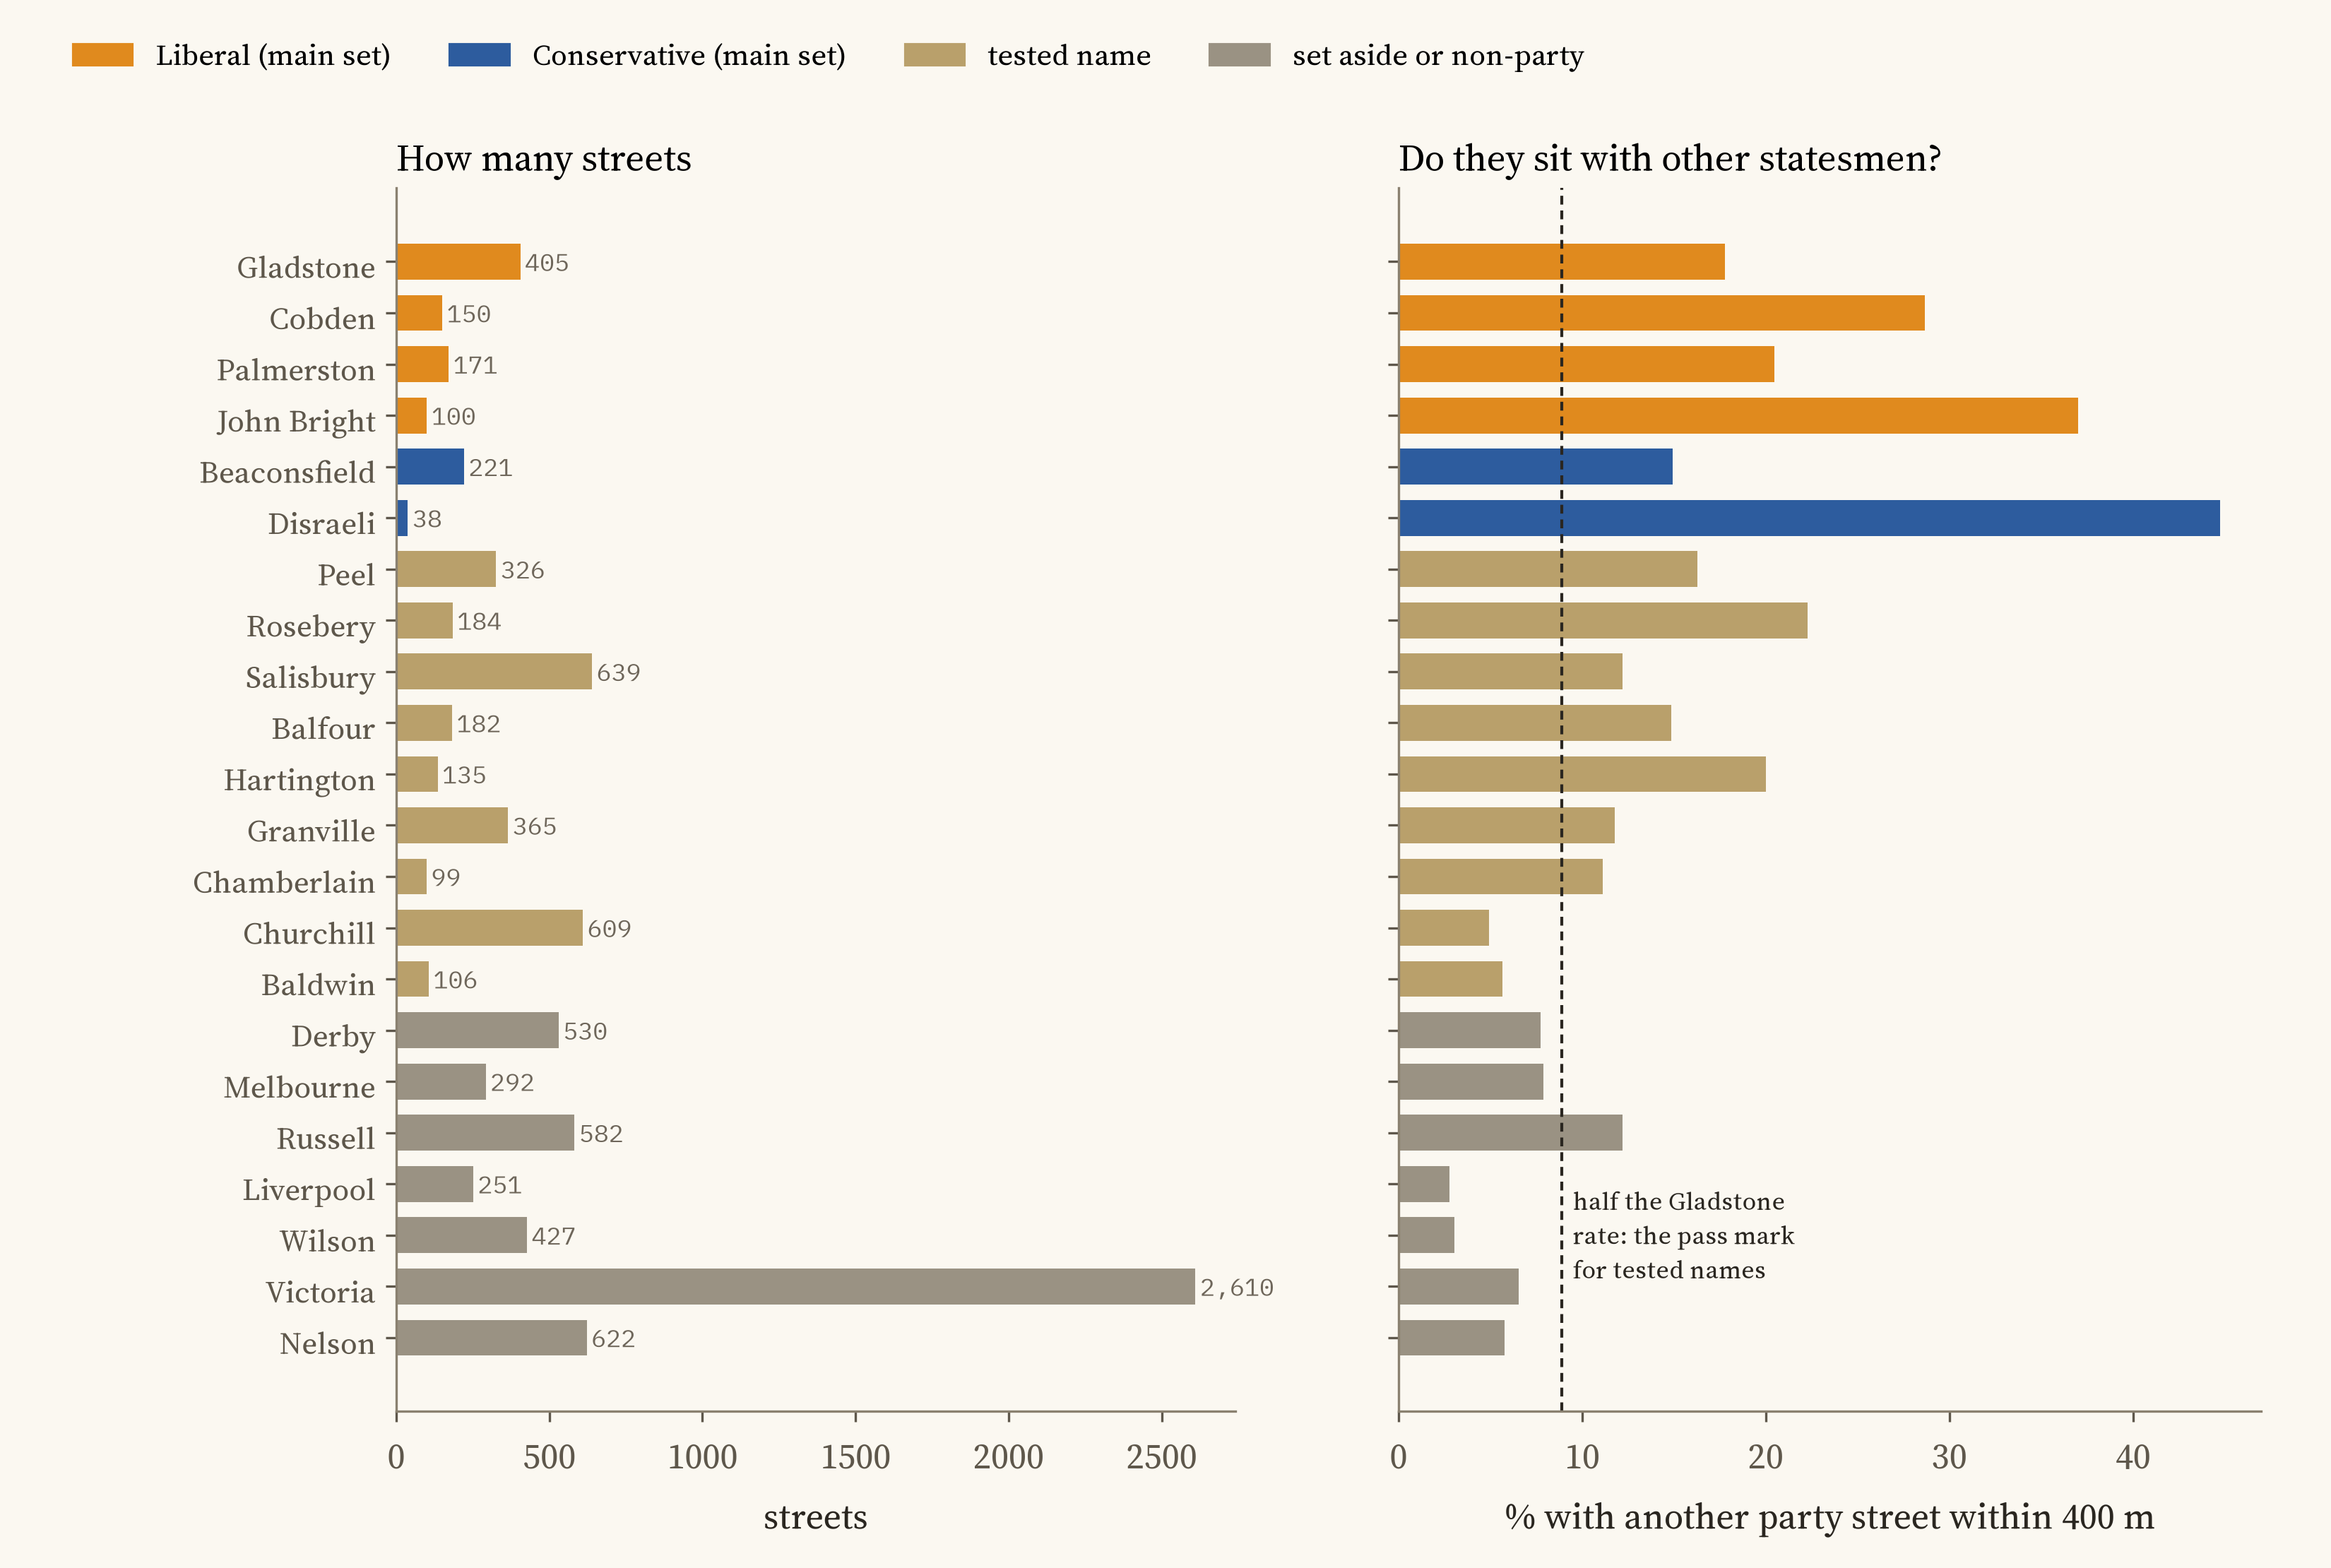
\includegraphics[width=\textwidth]{f_names.png}
\caption{Streets per name (left) and the share with a main-set party street of another name within 400 m (right). The dashed line is half the Gladstone rate, the pre-set pass mark for tested names. N = 15,593 streets in all.}\label{fig:names}\end{figure}

\subsection{Towns}
Towns are Wikidata settlements typed as towns or cities with a stated population of at least 3,000 (CC0). Each street is assigned to the town with the smallest ratio of distance to a radius that grows with population, $r = \max(3, 1.5\sqrt{\text{pop}/10{,}000})$ km, provided the distance is within $r$; all of Greater London is treated as London. 86.6\% of streets fall in a town. Present-day population is a proxy for size, not the Victorian population, which the data do not include.

\subsection{Elections}
Constituency results for every general election from 1832 to 2024 come from the open dataset of an earlier study, built from the UK Parliament results file (compiled from \citealp{craig1989,craig1974}) and House of Commons Library data, with candidates grouped into party families. A constituency is linked to a town when its name, after removing direction and division words (North, East, Central, Burghs, Boroughs, District), is the town's name, or begins with it followed by a ward name (Birmingham Bordesley, Liverpool Everton, Glasgow Govan); two-town seats (Penryn and Falmouth) link to both; a short alias list handles names such as The Hartlepools and Great Grimsby; county divisions named after counties are excluded, as are university seats and Ireland. Where two towns share a name the nearer to the seat's point is used. In London, every seat whose point lies in Greater London is London's. All 298 linked towns and their seats were read by eye (data file \texttt{links.csv}); the review found and removed one systematic error (the county divisions of Durham, matched at first to Durham city). 197 towns were parliamentary boroughs in 1868 to 1880.

The town's Liberal vote share is the Liberal family's share of Liberal plus Conservative and Liberal Unionist votes in its contested seats at each general election from 1868 to 1900, averaged over elections. Liberal Unionists are counted with the Conservatives, their allies from 1886. In two-member seats each elector had two votes, so shares are shares of votes cast. The alternative measure is the share of the town's seats won by Liberals, counting uncontested returns. For the placebo, the same linking gives each town's Liberal and Labour shares of all votes in the general elections of 1945 to 1970.

\subsection{Battle streets}
Streets named after battles, with the battle's date, come from an earlier study of the same OpenStreetMap data, with the same town assignment applied here. They give a count of each town's commemorative Victorian streets and a rough clock: Crimean battle streets (1854 to 1856) were mostly named in the 1850s, Boer War streets around 1900.

\section{Research design}
\subsection{Analysis plan}
The analysis plan was written in the project notes before any outcome model was run, after only the raw files and name counts had been examined. It fixed the hypotheses, the name sets, the units, the main specification, the robustness checks and what would count against the hypothesis. Everything reported as planned below was run as written; additions are labelled exploratory.

\textbf{H1 (main).} Across towns, the Liberal share of a town's party-political street names rises with the Liberal share of the town's vote at general elections from 1868 to 1900.

\textbf{H2 (timing).} Within towns, Gladstone and Beaconsfield streets lie at the same distance rank as late Victorian battle streets, between Crimean and Boer War streets; Labour names lie beyond First World War streets.

\textbf{H3 (Labour, secondary).} Towns with streets named after Labour figures had higher Labour vote shares from 1945 to 1970.

\subsection{Main specification}
The unit is the party-political street in the main set, in a town with a Victorian vote share. For street $i$ in town $t$ in region $g$,
\[ \text{Liberal}_{it} = \alpha + \beta\, V_t + \gamma \log \text{pop}_t + \delta \log(1+\text{royal}_t) + \theta\, \text{trad}_{i} + \mu_g + \varepsilon_{it}, \]
where $\text{Liberal}_{it}$ is 1 for a Liberal name and 0 for a Conservative one, $V_t$ is the town's Liberal vote share in units of 10 percentage points, $\text{royal}_t$ is the number of streets named Victoria, Albert or Alexandra (a proxy for the size of the town's Victorian street stock), $\text{trad}_i$ marks a traditional street word, and $\mu_g$ are fixed effects for the nine English regions, Wales and Scotland. Because streets in a town share their town's vote, standard errors are clustered by town \citep{cameron2015,abadie2023}. $\beta$ is the change in the probability that a party street is Liberal per 10 points of Liberal vote. Apart from the street-level street-word control, the linear probability model is a town-level regression of the Liberal share of names weighted by the number of party streets, so towns with many party streets count for more. The plan chose this weighting before the outcome was seen, because a share computed from one or two streets is very noisy; but H1 is a statement about towns, and the unweighted town-level regression, which answers it with every town counting equally, is reported as the first alternative and should be read alongside the main estimate. A binomial logit is also reported.

\subsection{Alternative specifications, placebos and robustness}
The plan specified: a binomial logit with standard errors clustered by county; an unweighted town-level regression on the Liberal share of names for towns with at least two party streets (HC3 errors), also without influential towns (Cook's distance above $4/n$); the share of seats won; the vote of 1868 to 1880 and of 1885 to 1900 separately; no controls; a control for battle streets; and parliamentary boroughs of 1868 only.

Two placebos. The first replaces the Victorian vote with the Liberal and the Labour shares of 1945 to 1970. If names were chosen with contemporary politics in mind, the later vote should predict them less well than the Victorian vote; if the later vote predicts them as well, the association more likely reflects a lasting local political culture than naming that followed the votes of the time. The second asks whether the Liberal vote predicts non-political Victorian commemoration (royal streets and battle streets) in town-level Poisson models with log population and region. A positive association would suggest that Liberal towns simply built more commemorative streets.

Robustness: randomisation inference, shuffling town vote shares within regions 2,000 times; leaving out each region in turn; dropping London and dropping the five towns with most party streets; and the measurement choices: a 600 m joining rule, town radii 0.7 and 1.4 times the default, the extended name set, Peel added as a Conservative, traditional street words only, counting same-party streets within 300 m of each other in a town once (builders named groups together, so streets are not independent), leaving out Gladstone, and England and Wales only.

The plan stated what would count against H1: a coefficient at or below zero, a confidence interval including zero with a point estimate under 1 point per 10 points of vote, or a later-period placebo as strong as the main estimate.

\subsection{Timing and Labour}
For H2, each party, Labour or battle street (battle streets with traditional street words only) is ranked by distance from its town's Wikidata point among all such streets in the town, in towns with at least three; the rank runs from 0 at the centre to 1 at the edge. Group means come with town-cluster bootstrap intervals (1,000 draws). For H3, a town-level linear probability model of having any Labour-named street on the Labour share of 1945 to 1970, log population, Victorian street stock and region (HC3 errors), with a logit alongside, then adding the Victorian Liberal vote.

\subsection{Threats to inference}
Three threats deserve explicit treatment. The first is confounding by town character. Liberal towns differed from Conservative ones in religion, industry and the timing of their growth, and any of these could shape naming without politics playing a part. The region fixed effects remove broad differences, the battle-street and royal-street counts proxy for the size and date of the Victorian street stock, and the later-period placebo asks whether a durable left-leaning character, rather than the vote of the time, explains the names. None of these removes confounding by unmeasured characteristics such as Nonconformity, and the results are interpreted as associations.

The second is measurement error. Both the names and the votes are noisy measures of what matters: the names include some streets that commemorate other people, and the town vote is an average over seats whose boundaries did not match the built-up area. Classical measurement error in the vote would bias the estimate towards zero; error in the outcome would reduce precision. The measurement checks vary the main construction choices one at a time to show how much the estimate depends on them.

The third is dependence. Streets in one town share a vote, so errors are clustered by town; streets laid out together by one builder are more alike than streets chosen independently, which the 300 m clustering check addresses; and towns near each other may share naming fashions, which leaving out each region in turn addresses. Randomisation inference provides a check that does not rely on asymptotic standard errors with few clusters per region.

\section{Results}
\subsection{A Liberal street culture}
The main set contains 826 Liberal and 242 Conservative party streets, a Liberal share of 77.3\%. Gladstone alone has 405 streets, more than Beaconsfield and Disraeli together (221 and 38). Cobden (150), Palmerston (171) and John Bright (100) follow (Figure~\ref{fig:map}). Liberal names are spread across the industrial north, the Midlands, South Wales and the south coast; Conservative names are thinner and concentrated in London, which has 41 of them against 62 Liberal names, more Conservative names than any other town. Scotland (67 Liberal, 10 Conservative) and Wales (43 and 7) are the most Liberal in their names, as they were in their votes.

\begin{figure}[tbp]\centering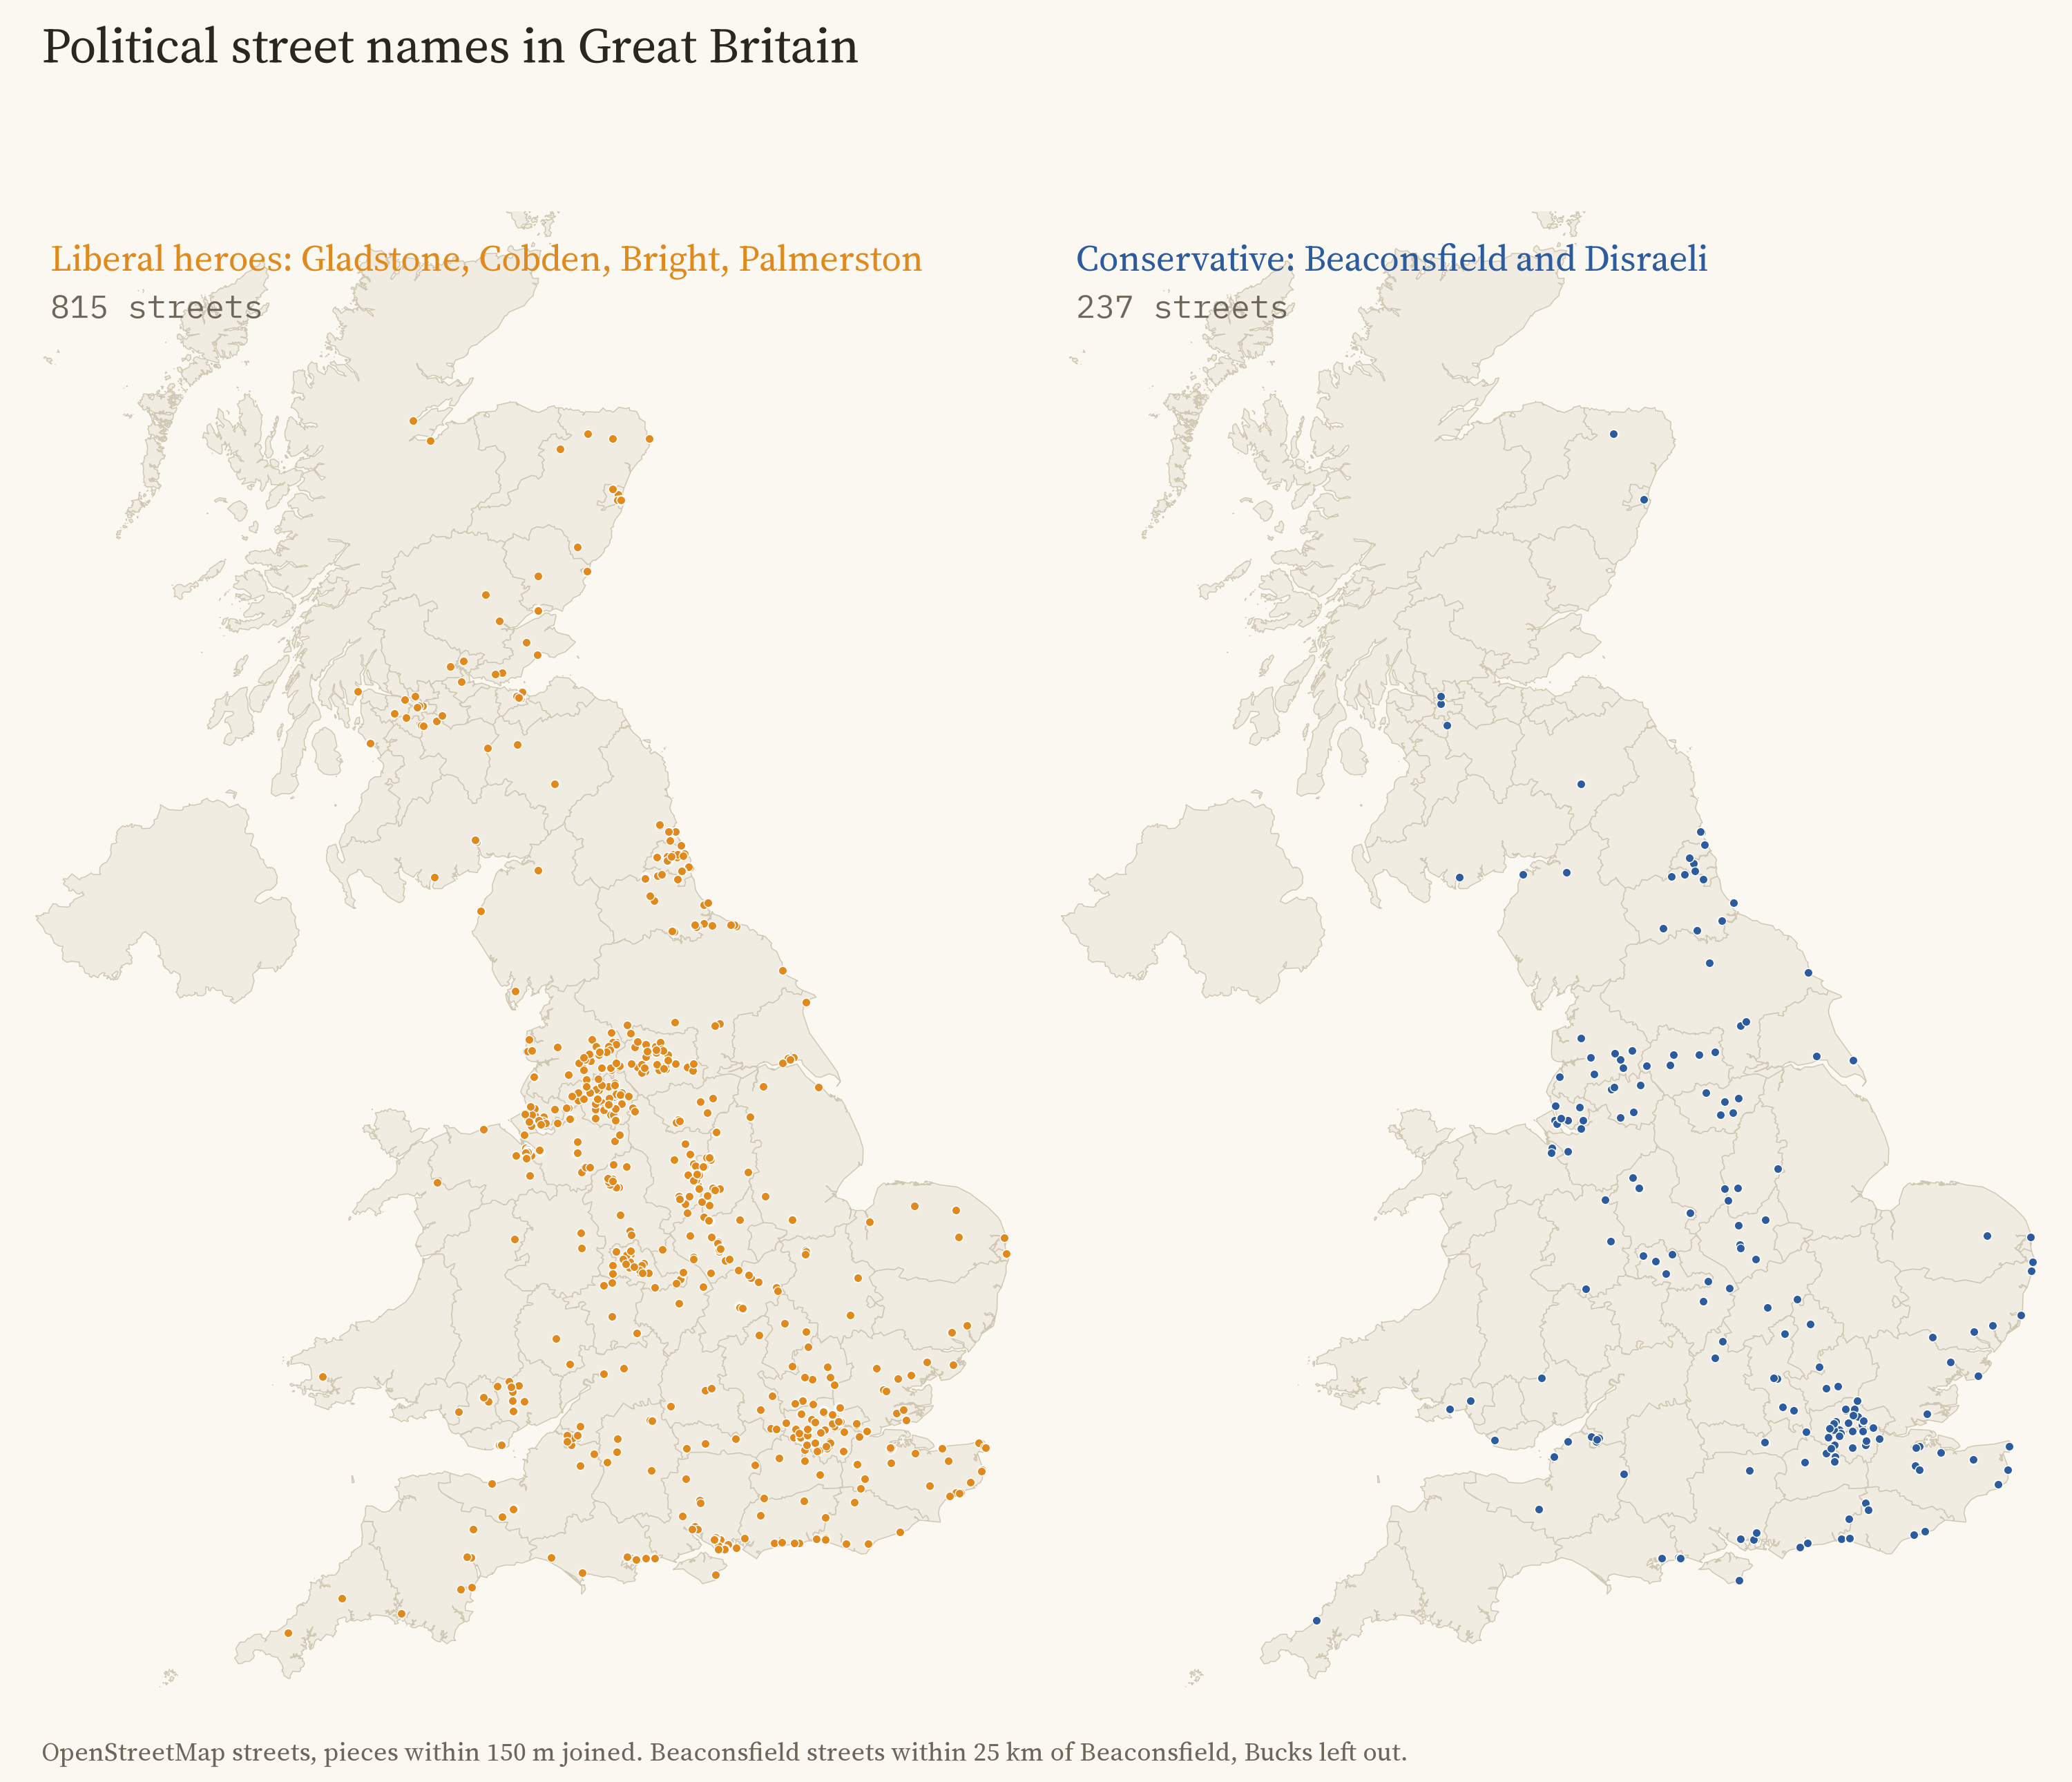
\includegraphics[width=0.92\textwidth]{f_map.png}
\caption{Main-set party streets in Great Britain: Liberal (left) and Conservative (right) names.}\label{fig:map}\end{figure}

The Liberal dominance of names is far larger than the Liberal lead in votes: across the sample towns the average Liberal share of the two-party vote is 52.6\% (standard deviation 11.1 points), but the average party street is Liberal with probability 0.75. Commemorative naming was not a mirror of the vote. Table~\ref{tab:region} gives the mix by region.

\subsection{Main result}
In the main model, each 10 points of Liberal vote share is associated with a 5.9 point higher probability that a party street is Liberal (95\% CI 0.4 to 11.4, $p=0.035$; N = 610 streets in 160 towns; Table~\ref{tab:main}). Moving from a town at 40\% Liberal to one at 60\% goes with 11.8 more points of Liberal names, and one standard deviation of vote with 6.6. The controls matter little: log population, the royal-street stock and the street word have coefficients close to zero, and the coefficient without any controls is 4.5 points (0.5 to 8.6). Figure~\ref{fig:towns} shows the town-level picture: a cloud with a gentle slope, with Blackburn (37\% Liberal vote, 5 Liberal names and none Conservative), Liverpool (39\% Liberal, 14 to 4) and Birmingham (10 to 1) as reminders that Conservative towns, and Chamberlain's Unionist Birmingham, also named streets after Liberals.

\begin{figure}[tbp]\centering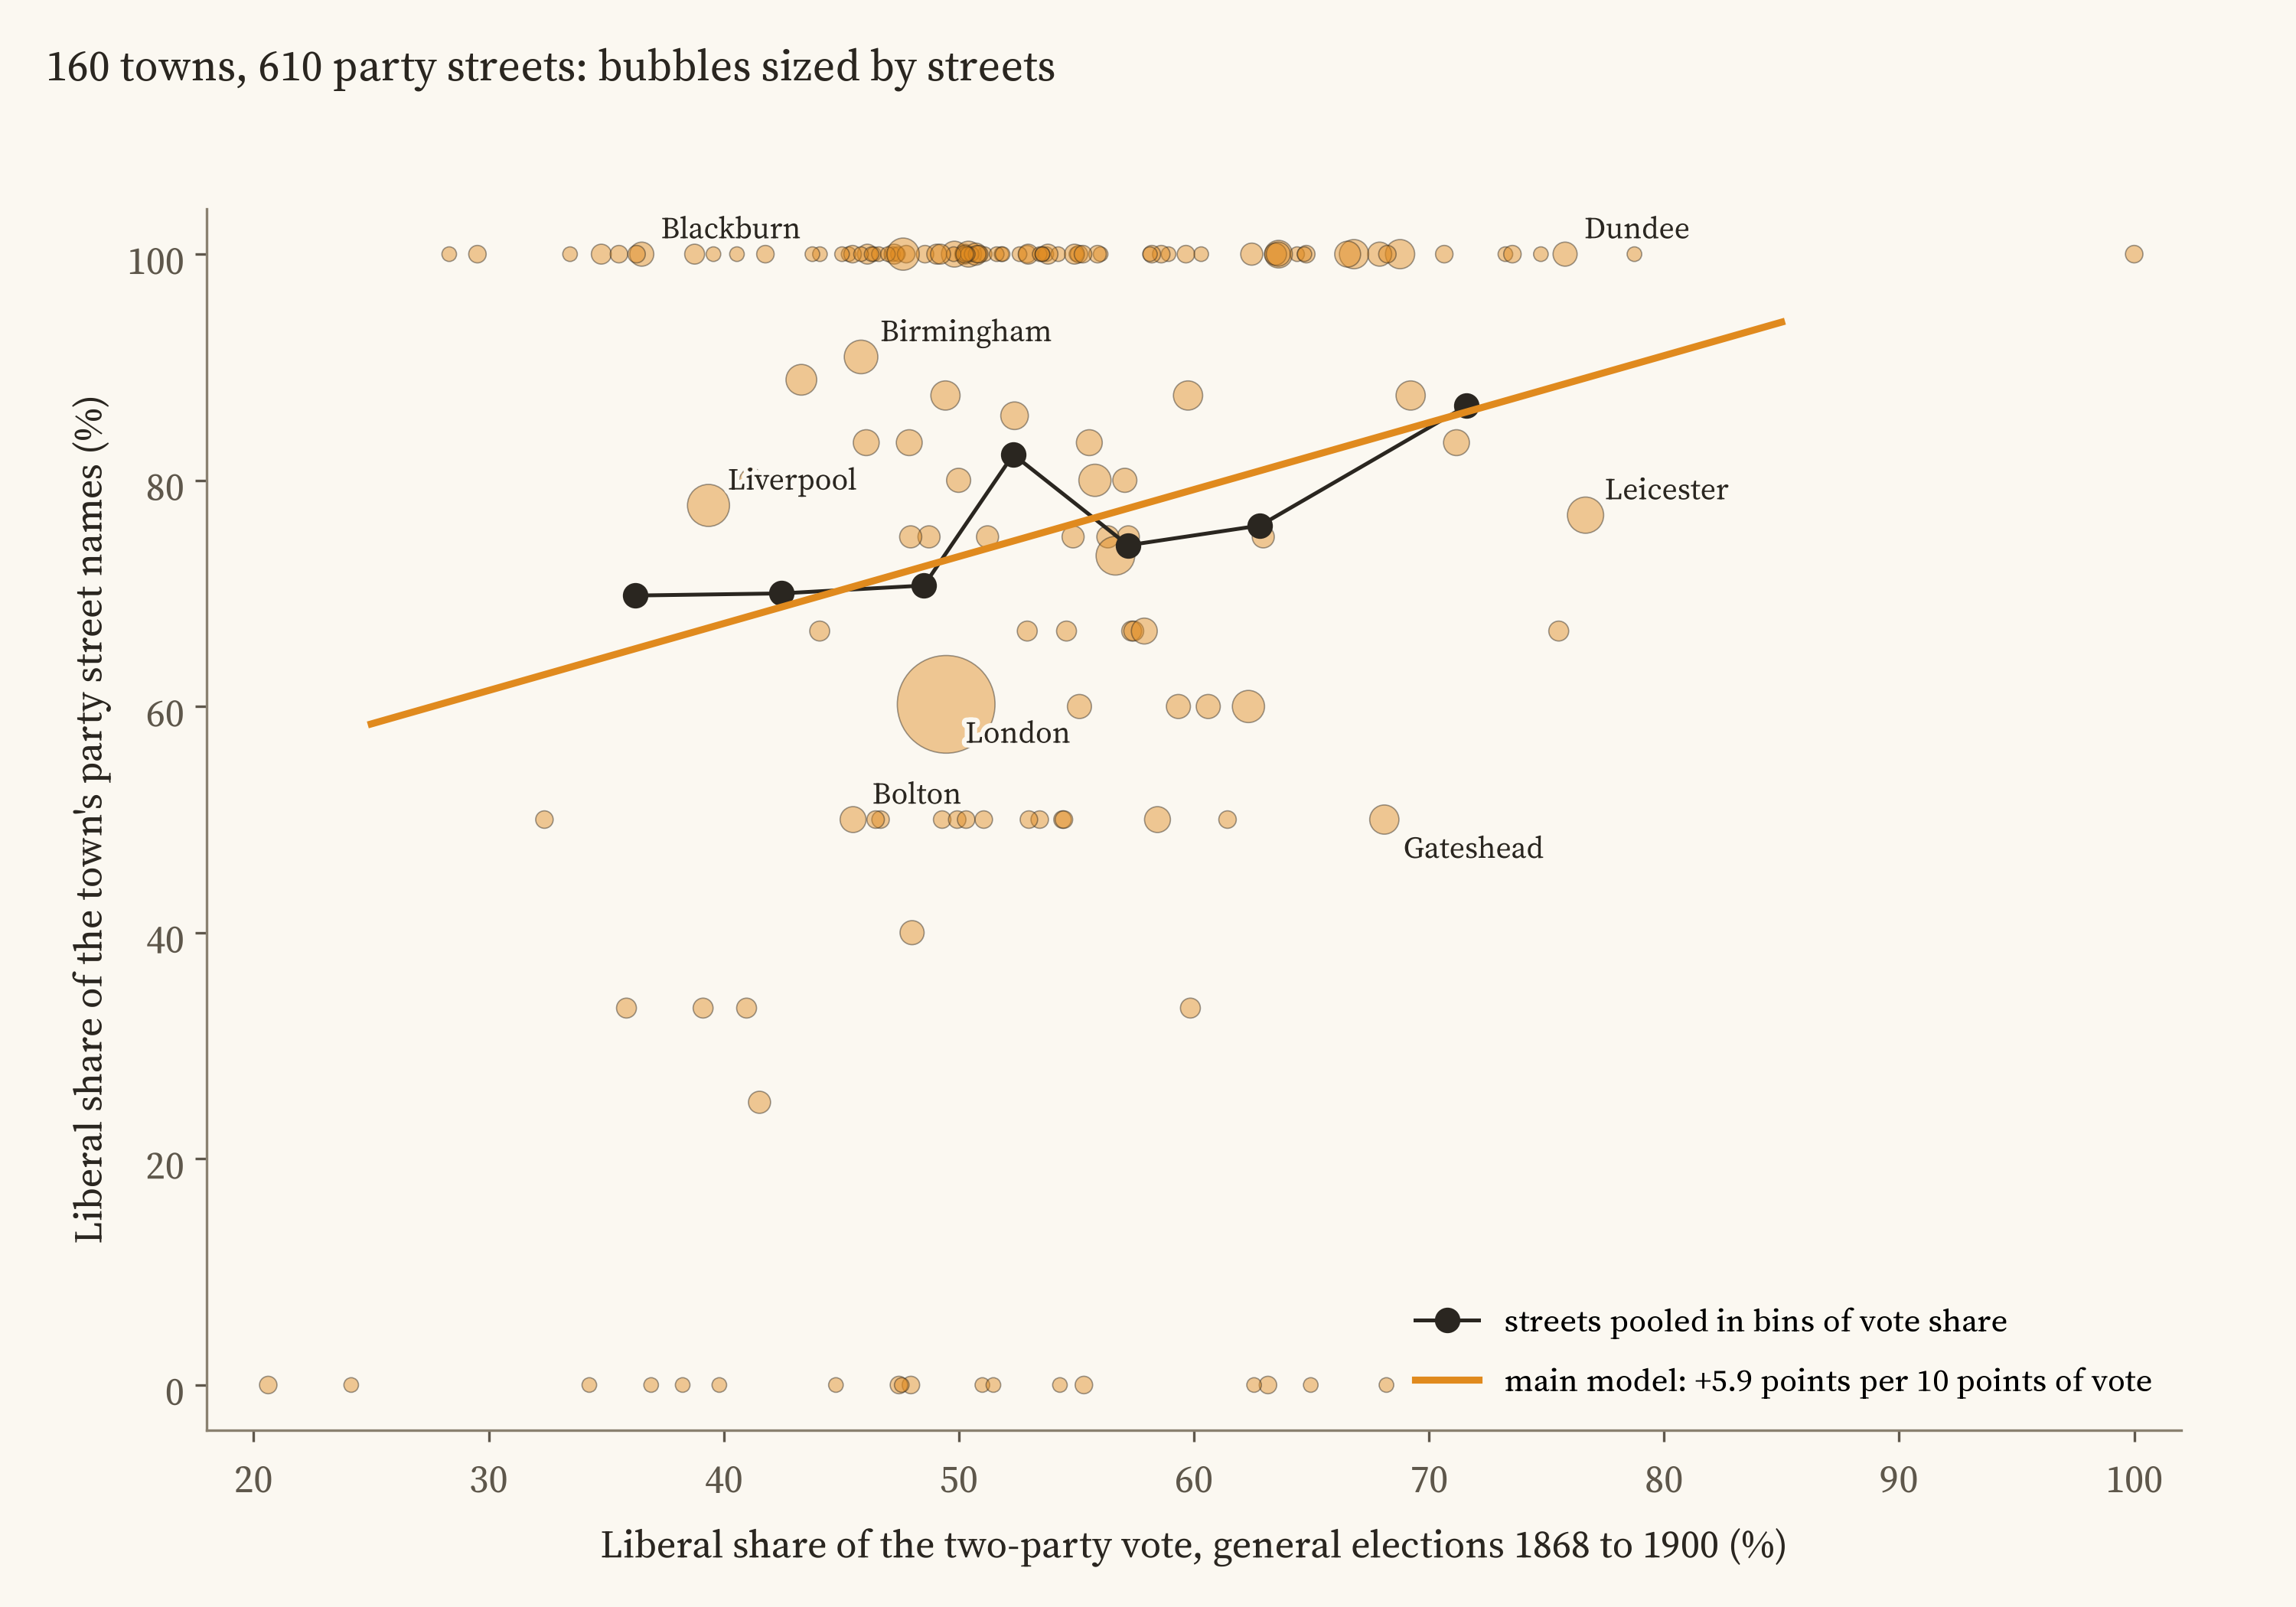
\includegraphics[width=0.95\textwidth]{f_towns.png}
\caption{Towns: Liberal share of the two-party vote 1868 to 1900 and the Liberal share of party street names. Bubbles are sized by the number of party streets; black points pool streets in bins of vote share; the orange line has the main model's slope. N = 160 towns, 610 streets.}\label{fig:towns}\end{figure}

\subsection{Alternative specifications}
The binomial logit gives a coefficient of 0.36 on the log-odds scale per 10 points (odds ratio 1.43, 95\% CI 1.03 to 1.99; average marginal effect 6.3 points), close to the linear model. The other alternatives are weaker (Table~\ref{tab:alt}). The unweighted town-level regression, which gives a town with two party streets the same weight as London, gives 6.3 points per 10 (-1.3 to 13.9, N = 108 towns), similar in size but not significant, and 5.4 without the 8 most influential towns. The share of seats won by Liberals shows no association (0.4 points per 10 points of seat share, -1.5 to 2.3). The vote of 1868 to 1880 alone (2.6, N = 489 streets in 103 towns) and of 1885 to 1900 alone (3.6) give positive but smaller and insignificant estimates, as does restricting to the parliamentary boroughs of 1868 (3.8, -2.4 to 10.0). Each of these is noisier than the main measure (fewer elections averaged, fewer towns, or a cruder outcome), but together they show that the main estimate is not robust to every reasonable choice. Adding the count of battle streets leaves it unchanged (6.2).

\subsection{Exploratory: which names carry the association}
This analysis was added after the planned models and is exploratory. Comparing each group of Liberal names with Beaconsfield and Disraeli separately, the association is 6.2 points per 10 points of vote for Gladstone (-1.4 to 13.8, N = 344), 9.9 for Cobden and Bright (1.1 to 18.6, N = 307) and 6.5 for Palmerston (-1.0 to 14.1, N = 261). The point estimates are similar, and only the radical free traders' names are individually distinguishable from zero. If anything, the names most closely tied to a cause, free trade and the repeal of the Corn Laws, follow the vote more closely than the names of prime ministers, which were more widely admired; but the differences between the three estimates are well within their uncertainty.

\subsection{Placebos}
The vote of 1945 to 1970 does not predict the Victorian names. On the same 597 streets in 151 towns with both votes, the Victorian Liberal vote gives 5.9 points per 10 (0.2 to 11.6), the Liberal share of 1945 to 1970 gives -1.4 (-9.2 to 6.4) and the Labour share 0.3 (-3.7 to 4.3); with the Labour share as a control the Victorian coefficient is 6.0 (Table~\ref{tab:placebo}). Victorian Liberal and later Labour shares are correlated across towns (r = 0.39, N = 245), so the null placebo is informative about one alternative: a lasting left-leaning character of the kind the later Labour vote measures does not account for the names. The later-period intervals are wide, however (the interval for the later Liberal share includes the main estimate), so the placebo is consistent with names that followed the vote of their own time rather than proof of it.

The second placebo is mixed. The Liberal vote does not predict the number of royal streets (incidence rate ratio per 10 points 1.04, 0.95 to 1.13) or of battle streets (0.94, 0.84 to 1.04), so Liberal towns did not simply commemorate more of everything. But they did have more party streets in total (1.16, 1.01 to 1.32, N = 297 towns). This is what partisan naming would produce if Liberal choices added Liberal names without removing Conservative ones, and it is consistent with the share result, but it also means the result rests on the extra Liberal names rather than on a visible deficit of Conservative names in Liberal towns.

\subsection{Robustness}
Randomisation inference, shuffling town vote shares within regions, gives a two-sided $p$ of 0.019 (38 of 2,000 draws as extreme). Leaving out each region in turn keeps the coefficient between 4.9 and 7.5 points. Without London the estimate is 5.9 (0.4 to 11.4); without the five towns with most party streets (London, Leicester, Birmingham, Liverpool and Bristol), 8.6 (3.3 to 14.0). The measurement checks leave the estimate between 5.2 and 8.8 points (Figure~\ref{fig:checks}, Table~\ref{tab:robust}): joining pieces within 600 m, smaller or larger town radii, the extended name set (1,427 streets in 213 towns: 5.2, 0.8 to 9.5), Peel as a Conservative, traditional street words only, and counting clusters of same-party streets once (447 units from 610 streets: 5.5, 0.3 to 10.8). Without Gladstone the estimate rises to 8.8, so it does not rest on one name. In England and Wales alone it is 5.2 (-0.6 to 10.9): Scotland's 10 towns, Liberal in both votes and names, add precision. 10 of 11 robustness estimates have intervals above zero.

\subsection{Exploratory checks added at review}
The checks in this subsection were added after the planned analysis, at an independent review, and are exploratory. They fall into four groups. First, does the result rest on one contestable name? Palmerston was a Whig-Liberal prime minister admired well beyond his party; without Palmerston streets the estimate is 6.5 points (0.2 to 12.8, N = 500). Bare ``Bright Street'' can be a surname; without all Bright streets it is 5.6 (-0.1 to 11.4). Keeping only plain street forms (dropping business parks, bridges, ``View'' names and bare names) gives 6.3 (0.8 to 11.8, N = 588). Second, and more important, without Beaconsfield the Conservative side is only Disraeli, and the estimate is 0.0 (-2.3 to 2.3, N = 481 streets of which 95.4\% are Liberal). Because Disraeli streets are so few, this check cannot rule out a proportionally similar effect (about one point per 10), but it shows that the association is carried by Beaconsfield names, which are rarer relative to Liberal names in Liberal towns. Beaconsfield is also a town and a house name; the route rule removes those near Buckinghamshire but cannot remove every non-political Beaconsfield. Third, the 150 m rule joins pieces by their first points only, so long streets mapped in several pieces can survive as two or more ``streets'': 145 of the 610 streets in the main sample have a same-named street in the same town within 600 m. The planned 600 m check above addresses this and gives the same answer, and errors clustered by town already allow for such dependence. Fourth, the constituency named after a town was a parliamentary borough before 1885, but from 1885 some towns are represented by county divisions named after them (Accrington, Barnsley and Sevenoaks, for example), whose voters included the surrounding countryside; the planned check restricted to the boroughs of 1868 is the cleanest test of the town hypothesis, and it gives a smaller, insignificant estimate.

\begin{figure}[tbp]\centering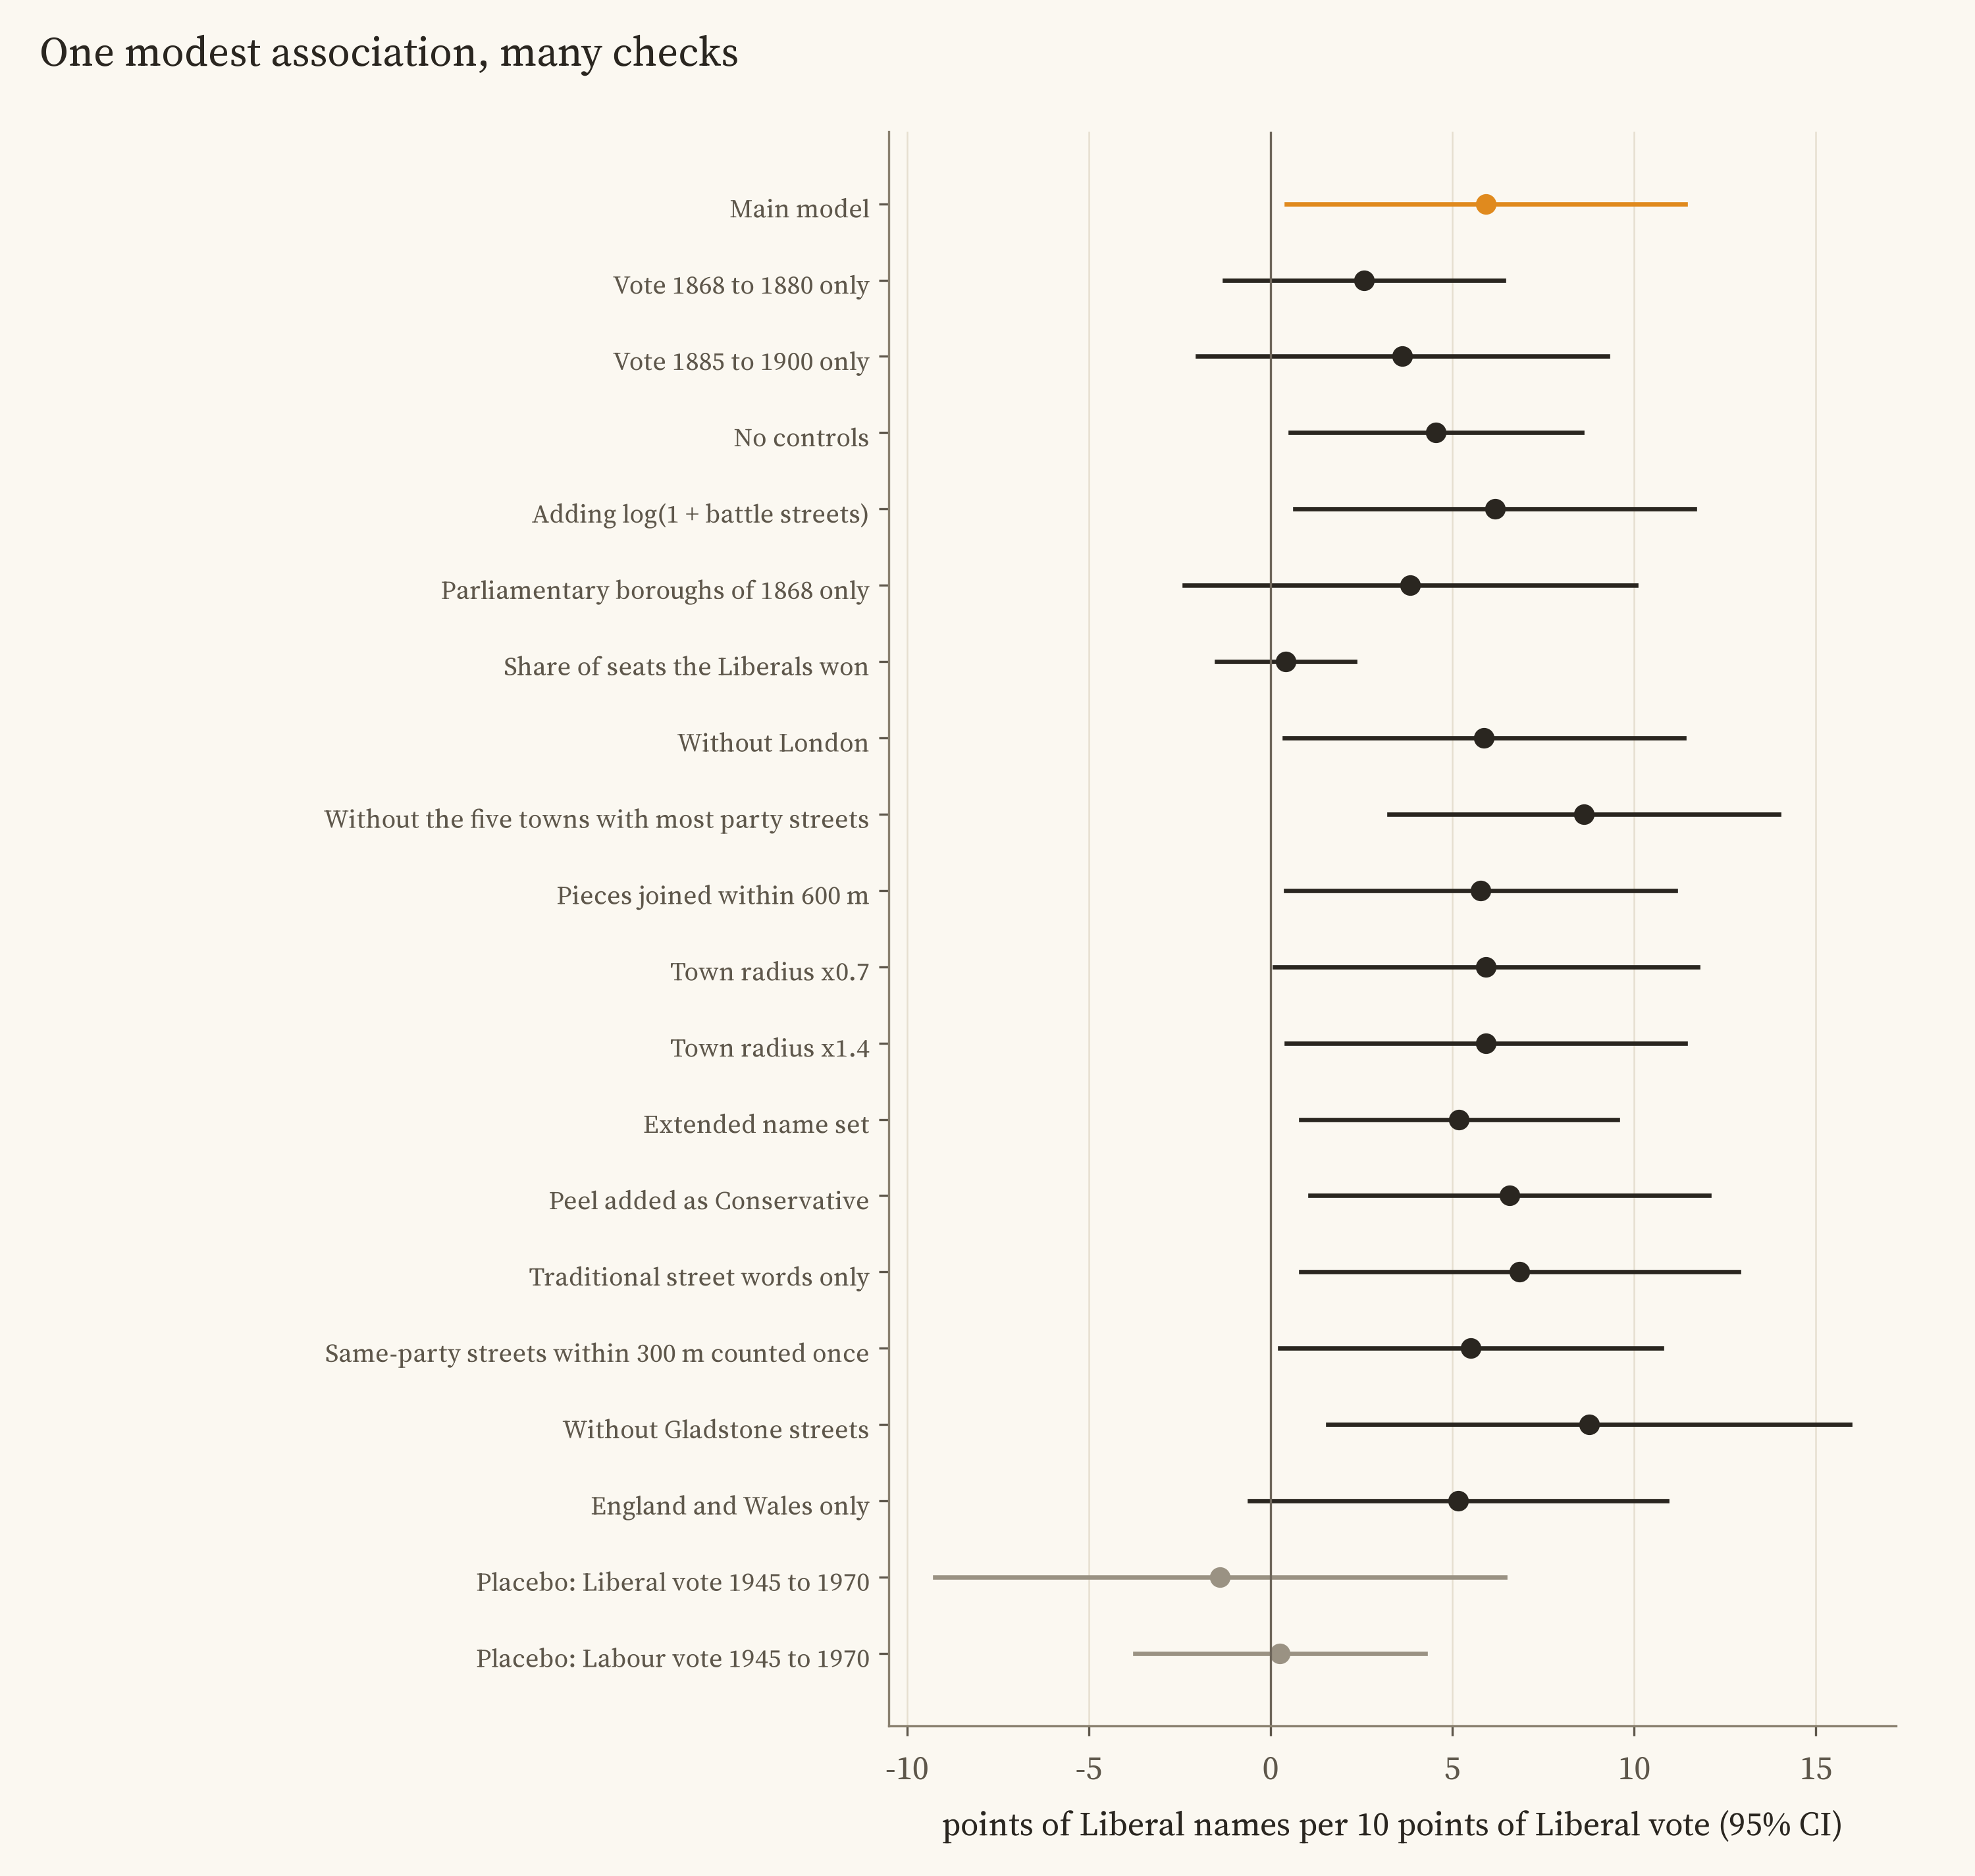
\includegraphics[width=0.9\textwidth]{f_checks.png}
\caption{The main estimate and the alternative, robustness and placebo estimates, with 95\% confidence intervals (points of Liberal names per 10 points of Liberal vote).}\label{fig:checks}\end{figure}

\subsection{Timing: when the political streets were built}
Within towns, Napoleonic battle streets sit at a mean distance rank of 0.49 and Crimean ones at 0.51; Gladstone streets at 0.58 (0.55 to 0.62), Beaconsfield and Disraeli streets at 0.58 (0.52 to 0.66) and Cobden, Bright and Palmerston at 0.59; Boer War streets at 0.61, First World War streets at 0.65 and Labour names at 0.72 (0.69 to 0.76; Figure~\ref{fig:clock}, Table~\ref{tab:timing}; 1,634 streets in 230 towns). As H2 predicted, the political names sit between the Crimean and Boer War streets: they were mostly laid out in the late Victorian decades, the period of the vote measure. Paired within towns, Gladstone streets lie farther out than Crimean streets in 38 of 61 towns with both, and nearer the centre than Boer War streets in 21 of 33; Gladstone and Beaconsfield streets are level (30 of 60). The clock is coarse \citep{whitehand1972}: towns grew along roads and railways, not in rings.

\begin{figure}[tbp]\centering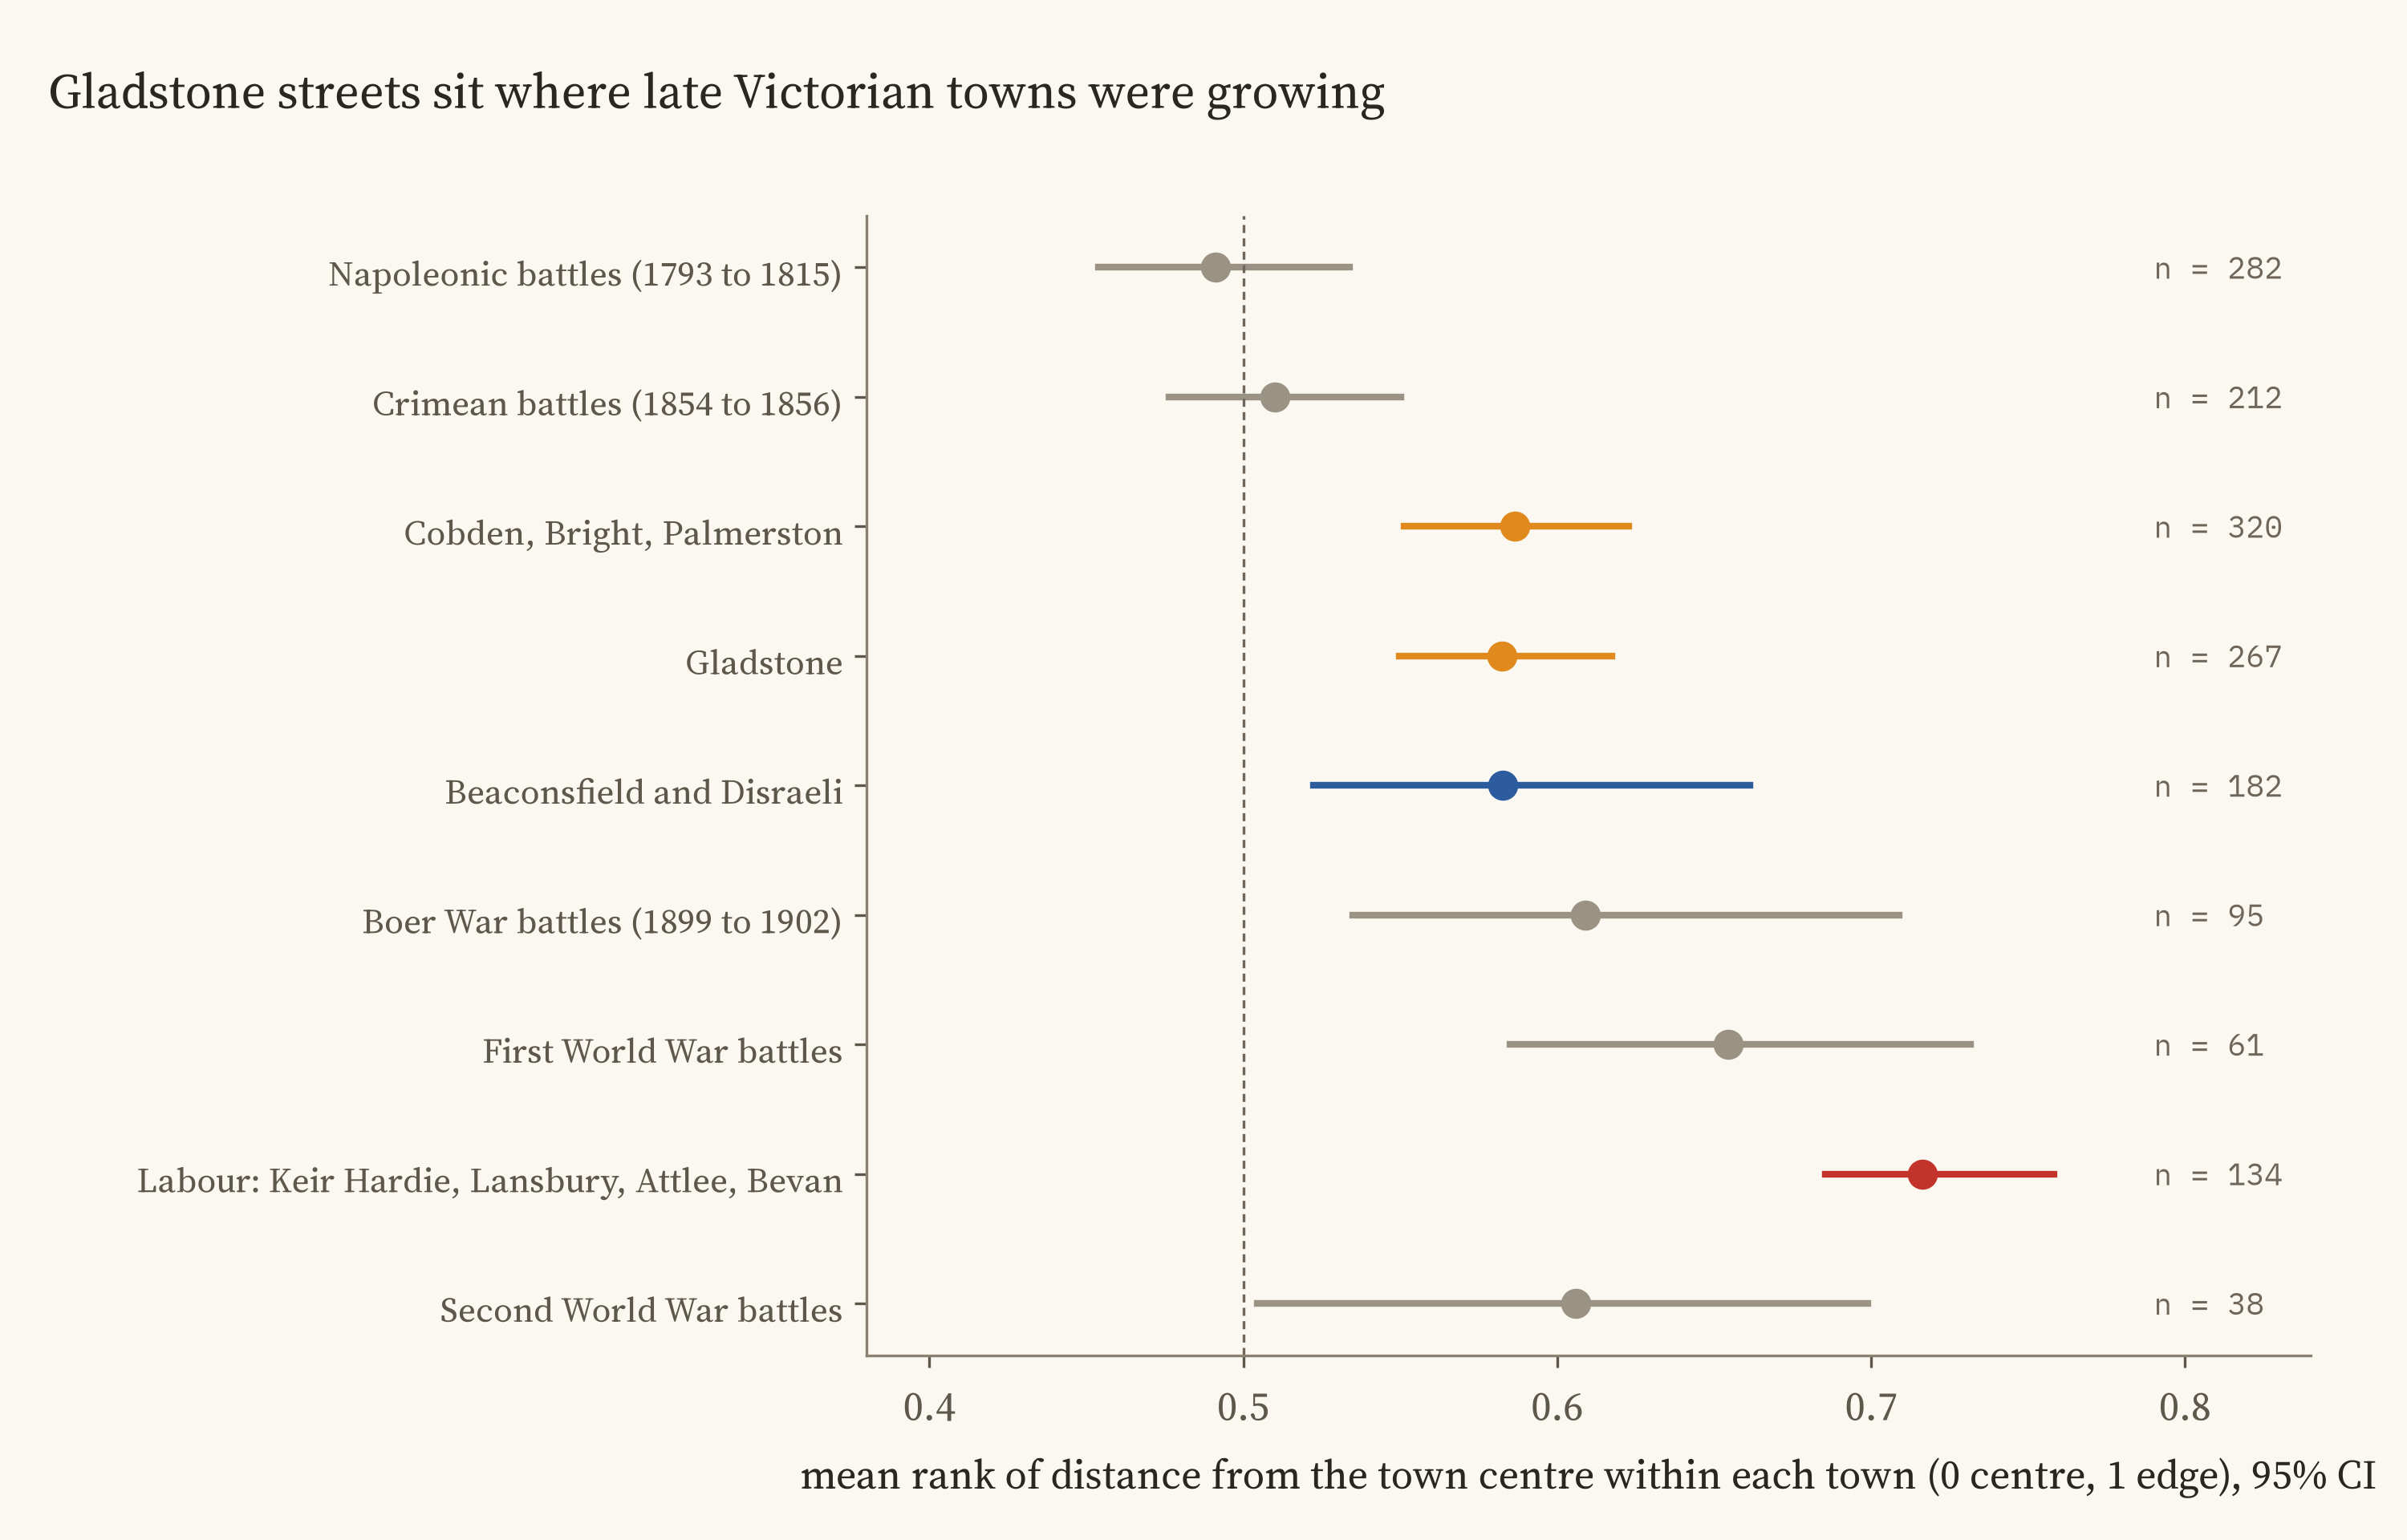
\includegraphics[width=0.92\textwidth]{f_clock.png}
\caption{Mean within-town rank of distance from the town centre (0 centre, 1 edge) for party, Labour and battle streets, with town-cluster bootstrap 95\% intervals.}\label{fig:clock}\end{figure}

\subsection{Labour names}
There are 205 streets named after Keir Hardie (40), Lansbury (85), Attlee (72) and Aneurin or Nye Bevan (8); bare Bevan and Hardie fail the co-location test and are left out. Greater London has more Lansbury names than anywhere else (14 of 85, including the Lansbury estate in Poplar), and Labour names cluster in the coalfields of South Wales, County Durham and central Scotland (Figure~\ref{fig:labour}). Of 245 towns with a 1945 to 1970 vote, 31 have a Labour-named street: 3\% of the least Labour quarter of towns and 28\% of the most Labour quarter. In the linear model each 10 points of Labour vote goes with 4.2 points higher probability of a Labour street (-0.1 to 8.6; logit $p=0.041$), and adding the Victorian Liberal vote changes little (its own coefficient 1.2, -4.4 to 6.8; Table~\ref{tab:h3}). The evidence for H3 is suggestive, not conclusive, and the Labour names are too few to say whether they were chosen by Labour councils, which the data do not record.

\begin{figure}[tbp]\centering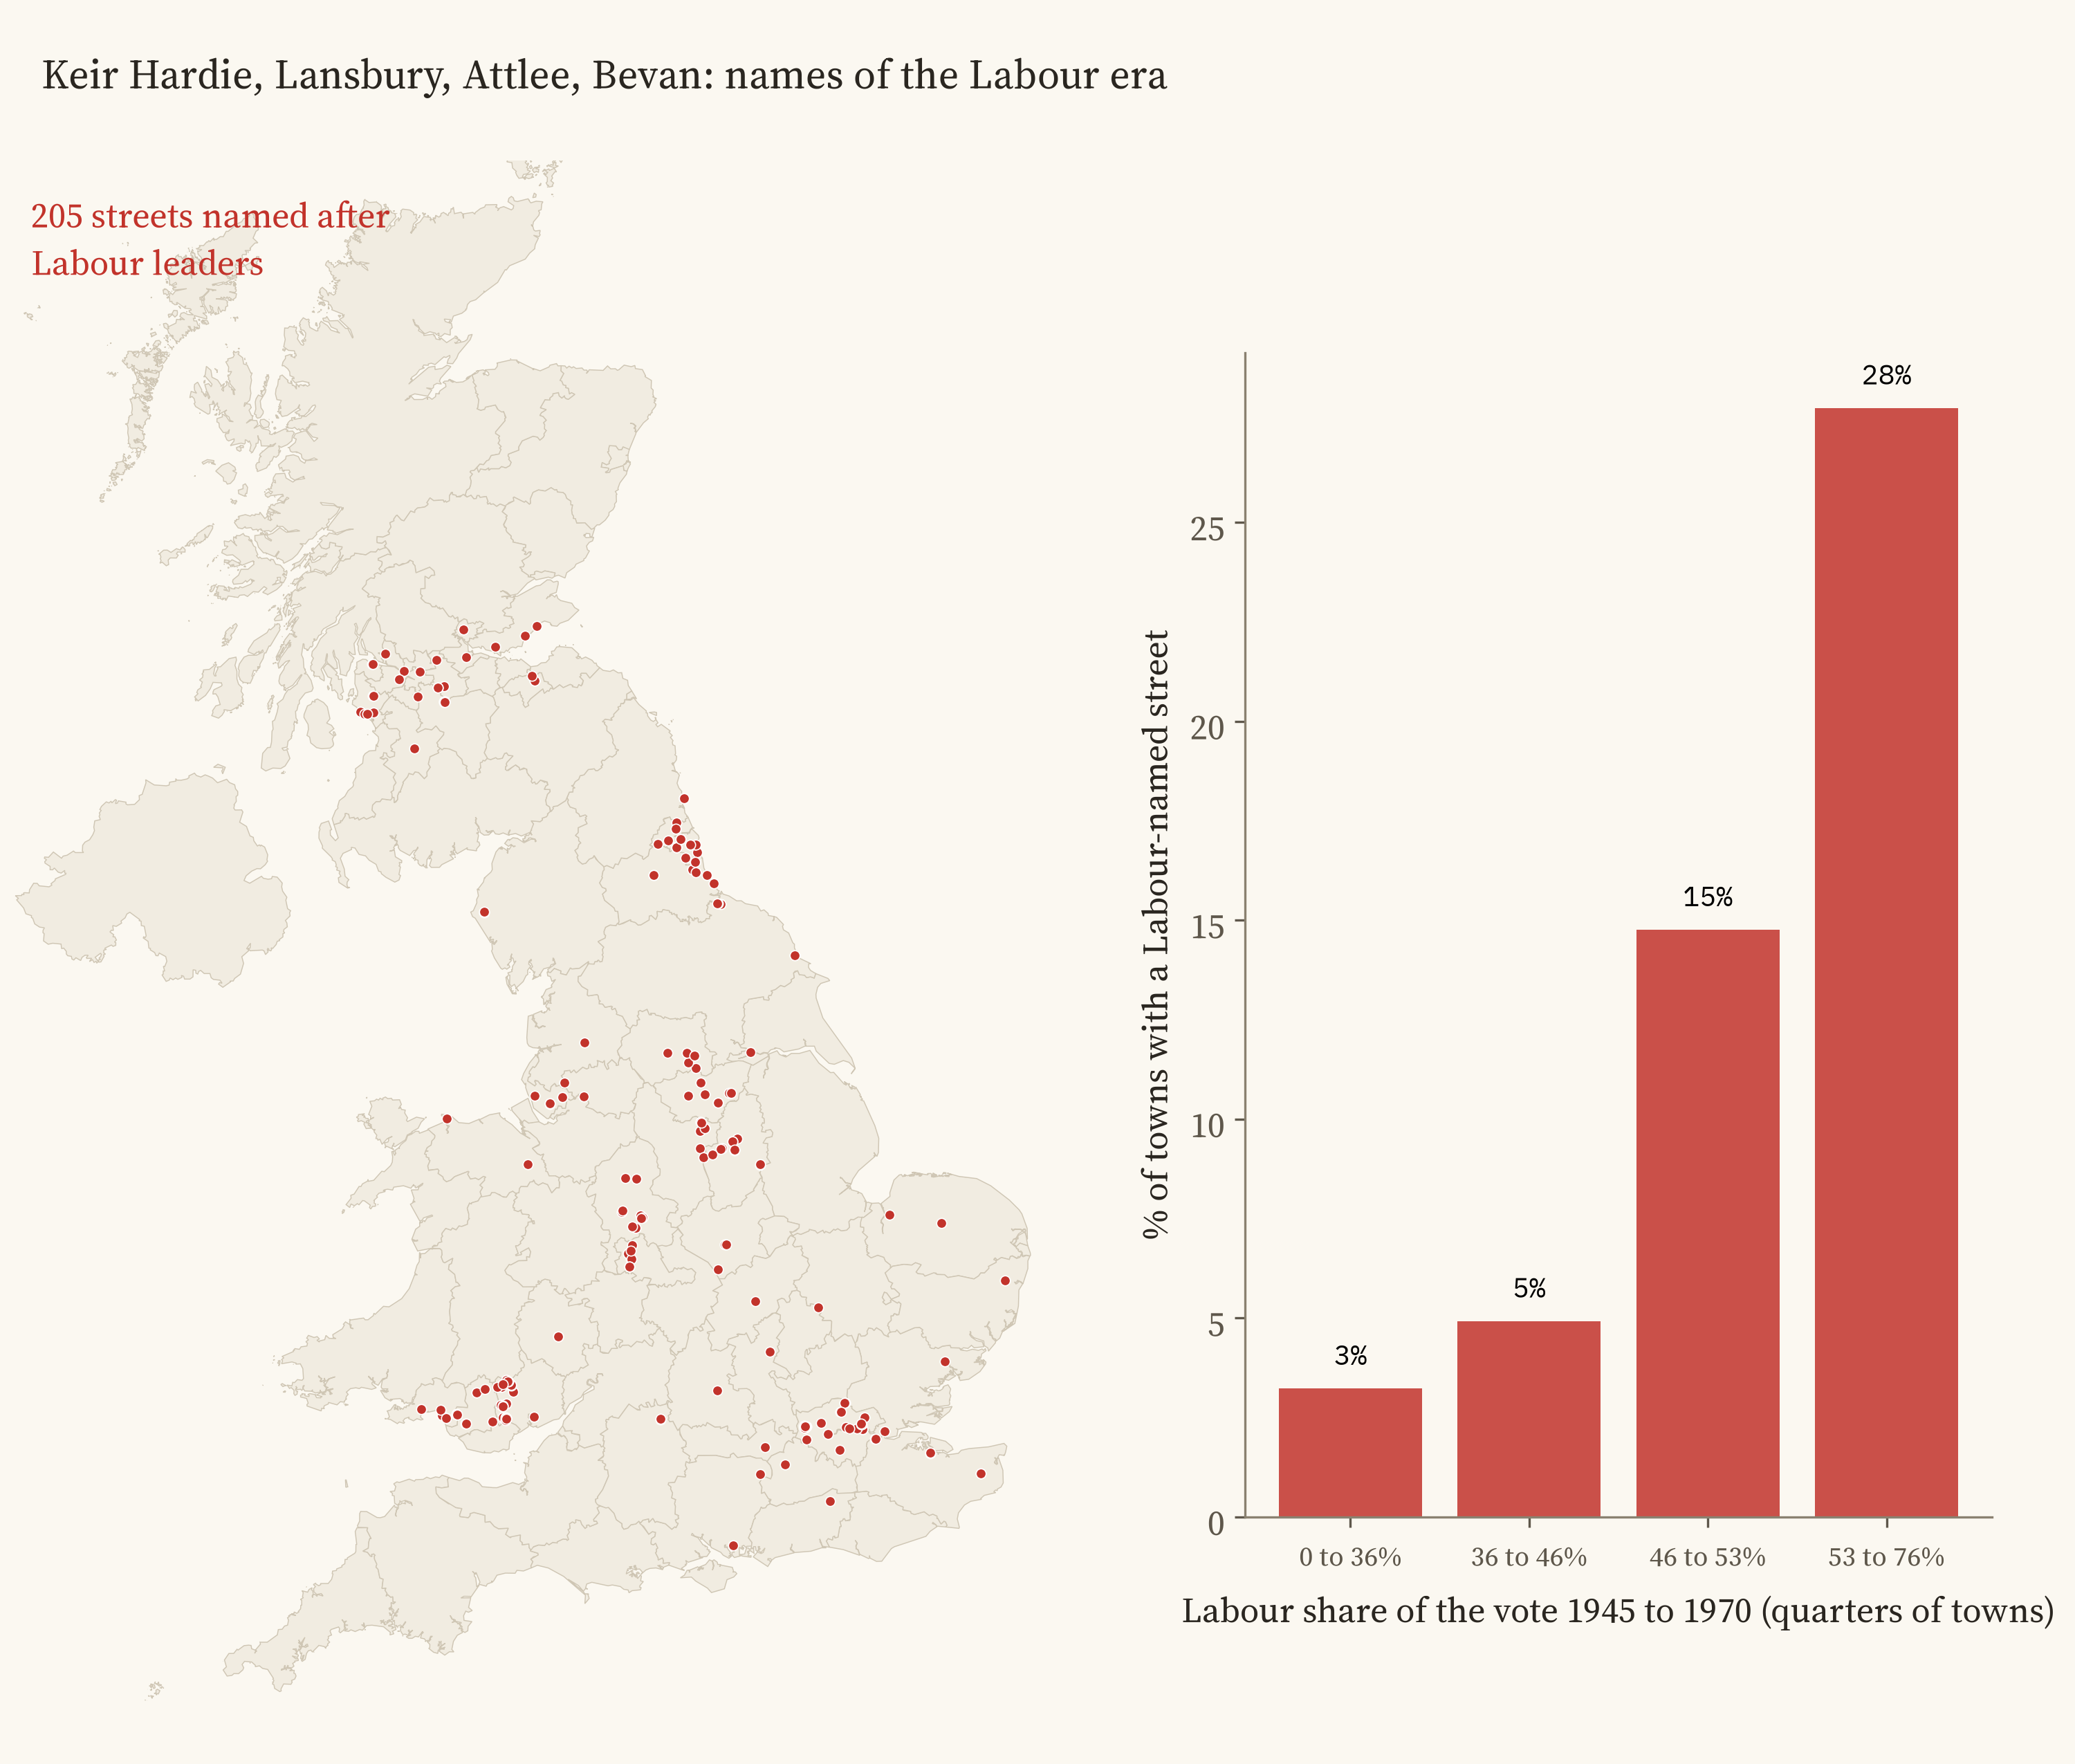
\includegraphics[width=0.92\textwidth]{f_labour.png}
\caption{Streets named after Labour leaders (left) and the share of towns with one, by quarter of the Labour vote 1945 to 1970 (right; N = 245 towns).}\label{fig:labour}\end{figure}

\section{Discussion}
\subsection{What the names say}
The first finding is not about local politics at all. Across Britain, party street names were overwhelmingly Liberal: Gladstone, Cobden, Bright and Palmerston outnumber Disraeli and Beaconsfield by more than three to one, in Conservative as well as Liberal towns. That is consistent with the historians' picture of a popular Liberal culture with a cult of its leaders \citep{biagini1992,matthew1986} and of free trade as a national faith rather than a party one \citep{howe1997,trentmann2008}. Cobden and Bright names in Tory Lancashire towns such as Blackburn are a reminder that in the cotton towns the Anti-Corn Law League's heroes were local heroes, whatever the town's vote \citep{joyce1980}. Conservative commemoration may simply have taken other forms, such as the Primrose League's habitations, badges and Primrose Day \citep{pugh1985}. London is the exception, with a Conservative share of names much closer to its Conservative vote than elsewhere, which fits accounts of a distinctive popular Conservatism in the capital \citep{windscheffel2007}.

The asymmetry itself is worth explaining. One possibility is supply: Liberal heroes were more numerous and more varied (Gladstone, Cobden, Bright, Palmerston, later Rosebery), while the Conservative pantheon of the period was dominated by one man, and Salisbury, the other Conservative prime minister of the age, shared his name with a city. Another is the social position of those who laid out streets. Builders, small developers and freehold land societies may have been drawn disproportionately from the Nonconformist lower middle class that formed a core of urban Liberalism \citep{vincent1966}, while Conservative landowners, whose estates were also developed, more often used family names and titles than the names of party leaders. A third is that Liberal political culture placed more weight on the cult of named leaders and causes, whereas popular Conservatism appealed to Crown, Church and Empire, which have their own street names (Victoria, Albert, Alexandra, Wellington, Nelson) that are not counted here as party names.

The second finding is that the partisan mix of names moved with the town's vote, but weakly. A town 20 points more Liberal had about 12 points more Liberal names. The estimate survives most checks, and the later-period placebo is null even though the later vote is correlated with the Victorian one, which is what naming in line with contemporary politics would produce. But the estimate is imprecise: without weights at the town level it is about the same size but no longer distinguishable from zero, it is absent with the share of seats won, and in exploratory checks it is carried by the relative scarcity of Beaconsfield names in Liberal towns. Its lower confidence bound is close to zero. A fair summary is that street names carry a faint trace of local partisanship on top of a strong national Liberal culture.

\subsection{Mechanisms the data cannot separate}
Several mechanisms could produce the association, and the data cannot tell them apart. Builders and freehold land societies in Liberal towns may have chosen Liberal names for their own reasons or to sell houses to Liberal buyers; Liberal-controlled councils may have approved or suggested names; or the same Nonconformist, industrial communities that voted Liberal may simply have admired Gladstone more, without any decision being political. The design is correlational: it shows that names and votes moved together across towns, not that votes caused names. Nor can it say whether a street was named when it was built or renamed later, though the timing evidence suggests most party names date from the late Victorian decades, and the traditional-street-word check (Street, Road, Terrace) gives the same answer.

\subsection{Limitations}
The street data are present-day names. Streets that were renamed, demolished in slum clearance or bombed are missing, and their losses were not random: inner-city terraces, where many Victorian political names stood, were cleared in large numbers after 1945. Losses that removed Liberal and Conservative names alike would not bias the share; losses that fell more on one party's names in towns of one political colour would, and the data cannot test this. OpenStreetMap's coverage is good in towns but not perfect \citep{haklay2010}. The name table cannot separate a Gladstone Road named after the statesman from one named after a local Gladstone family or Liverpool's Gladstone Dock; the co-location test shows that main-set names behave like commemorations as a group, not that every one is.

The town is a rough unit. Towns are assigned by distance to a Wikidata point with a population-based radius, using present population, which gives London a reach of more than 40 km (all streets in Greater London are London's in any case, and only one street in the main sample lies outside it); the vote is the average of the seats named after the town, which before 1885 often included two-member boroughs whose boundaries differed from the built-up area, and after 1885 included county divisions named after towns. Uncontested elections are missing from the vote measure; the seats-won measure includes them and shows no association. Regional fixed effects absorb broad differences, but other town characteristics (religion, industry, the date and scale of Victorian growth) are not measured and may drive both votes and names \citep{wald1983,pelling1967}. With 160 towns, and London contributing 103 of the streets, precision is limited.

Renaming is a further source of loss. In London the Metropolitan Board of Works, from 1857, and then the London County Council renamed many streets to bring order to the postal map, with a last large round in the late 1930s; towns that absorbed their neighbours could face the same problem of several Gladstone or Victoria Streets. A renamed political street is invisible here. If renaming fell on the commonest names, Gladstone and Victoria streets are undercounted relative to rarer names, which would understate the Liberal dominance of names rather than create it.

The analysis also leaves out Northern Ireland, where the party system differed, and county constituencies named after counties, whose voters lived mostly outside towns. The results apply to the towns of Great Britain that had seats named after them, which were the larger and older towns; whether the same pattern holds in the suburbs and small towns that were not separately represented cannot be tested with these data.

\subsection{Street names as data}
For research that uses street names as measures of culture \citep{oto2018,gutierrez2022,bancilhon2021}, the findings carry two lessons. First, the dominant signal in commemorative names may be national rather than local: almost every town named its political streets after Liberals. A local measure built from such names will mostly measure the size and age of a town's Victorian street stock unless it is expressed as a share, as here. Second, ambiguity is a first-order problem. Many of the names that look most promising (Salisbury, Derby, Melbourne, Russell) are mainly something else, and a measure that counted them would be dominated by noise. The co-location test used here, which asks whether a name keeps company with other commemorations of the same kind, is simple and transparent and could be applied to other commemorative sets.

\section{Conclusion}
Victorian Britain wrote its politics into its streets, but mostly in one direction. Gladstone, Cobden, Bright and Palmerston were commemorated across the country, in Conservative as well as Liberal towns, far more often than Disraeli. On top of that national pattern, towns that voted more Liberal named a slightly larger share of their political streets after Liberals, by about 6 points per 10 points of vote in the pre-specified model, an association that survives most robustness checks and a later-period placebo but not every reasonable alternative. Within towns, the political names sit in the late Victorian rings of growth, and Labour names in the estates beyond them. Street names are a usable, if faint, record of partisan memory, and the name table and code released with this paper allow the same test for other countries, periods and commemorative sets.

\section*{Data availability statement}
Data and code: Zenodo DOI https://doi.org/10.5281/zenodo.24092657. The interactive map is at \url{https://maps.tristanhotham.com/pm-streets/} and the repository at \url{https://github.com/Tristan-Hotham/pm-streets}. The street tables are derived from OpenStreetMap (ODbL); election results from the UK Parliament and House of Commons Library (Open Parliament Licence v3.0); settlements from Wikidata (CC0); boundaries from the ONS (OGL v3.0).

\section*{AI statement}
I wrote the text, with drafting and editing assistance from Claude (Anthropic), which also helped prepare the analysis code. I reviewed and checked all text and results.

\begin{thebibliography}{99}
\bibitem[Abadie et al.(2023)]{abadie2023} Abadie, A., Athey, S., Imbens, G. W. and Wooldridge, J. M. (2023) When should you adjust standard errors for clustering? \textit{Quarterly Journal of Economics} 138(1), 1 to 35.
\bibitem[Alderman(2000)]{alderman2000} Alderman, D. H. (2000) A street fit for a King: naming places and commemoration in the American South. \textit{The Professional Geographer} 52(4), 672 to 684. doi:10.1111/0033-0124.00256.
\bibitem[Alderman(2003)]{alderman2003} Alderman, D. H. (2003) Street names and the scaling of memory: the politics of commemorating Martin Luther King, Jr within the African American community. \textit{Area} 35(2), 163 to 173. doi:10.1111/1475-4762.00250.
\bibitem[Azaryahu(1996)]{azaryahu1996} Azaryahu, M. (1996) The power of commemorative street names. \textit{Environment and Planning D: Society and Space} 14(3), 311 to 330. doi:10.1068/d140311.
\bibitem[Azaryahu(1997)]{azaryahu1997} Azaryahu, M. (1997) German reunification and the politics of street names: the case of East Berlin. \textit{Political Geography} 16(6), 479 to 493. doi:10.1016/S0962-6298(96)00053-4.
\bibitem[Bancilhon et al.(2021)]{bancilhon2021} Bancilhon, M., Constantinides, M., Bogucka, E. P., Aiello, L. M. and Quercia, D. (2021) Streetonomics: quantifying culture using street names. \textit{PLoS ONE} 16(6), e0252869. doi:10.1371/journal.pone.0252869.
\bibitem[Bast and Buchhold(2017)]{bast2017} Bast, H. and Buchhold, B. (2017) QLever: a query engine for efficient SPARQL+Text search. In \textit{Proceedings of the 26th ACM International Conference on Information and Knowledge Management (CIKM)}, 647 to 656. doi:10.1145/3132847.3132921.
\bibitem[Biagini(1992)]{biagini1992} Biagini, E. F. (1992) \textit{Liberty, Retrenchment and Reform: Popular Liberalism in the Age of Gladstone, 1860 to 1880}. Cambridge: Cambridge University Press.
\bibitem[Cameron and Miller(2015)]{cameron2015} Cameron, A. C. and Miller, D. L. (2015) A practitioner's guide to cluster-robust inference. \textit{Journal of Human Resources} 50(2), 317 to 372.
\bibitem[Cox(1987)]{cox1987} Cox, G. W. (1987) \textit{The Efficient Secret: The Cabinet and the Development of Political Parties in Victorian England}. Cambridge: Cambridge University Press.
\bibitem[Craig(1974)]{craig1974} Craig, F. W. S. (ed.) (1974) \textit{British Parliamentary Election Results 1885 to 1918}. London: Macmillan. doi:10.1007/978-1-349-02298-4.
\bibitem[Craig(1989)]{craig1989} Craig, F. W. S. (ed.) (1989) \textit{British Parliamentary Election Results 1832 to 1885}, 2nd edn. Dartmouth: Parliamentary Research Services.
\bibitem[Dyos(1961)]{dyos1961} Dyos, H. J. (1961) \textit{Victorian Suburb: A Study of the Growth of Camberwell}. Leicester: Leicester University Press.
\bibitem[Gutiérrez-Mora and Oto-Peralías(2022)]{gutierrez2022} Gutiérrez-Mora, D. and Oto-Peralías, D. (2022) Gendered cities: studying urban gender bias through street names. \textit{Environment and Planning B: Urban Analytics and City Science} 49(6), 1792 to 1809. doi:10.1177/23998083211068844.
\bibitem[Haklay(2010)]{haklay2010} Haklay, M. (2010) How good is volunteered geographical information? A comparative study of OpenStreetMap and Ordnance Survey datasets. \textit{Environment and Planning B: Planning and Design} 37(4), 682 to 703. doi:10.1068/b35097.
\bibitem[Hanham(1959)]{hanham1959} Hanham, H. J. (1959) \textit{Elections and Party Management: Politics in the Time of Disraeli and Gladstone}. London: Longmans.
\bibitem[Hinde(1987)]{hinde1987} Hinde, W. (1987) \textit{Richard Cobden: A Victorian Outsider}. New Haven and London: Yale University Press.
\bibitem[Howe(1997)]{howe1997} Howe, A. (1997) \textit{Free Trade and Liberal England, 1846 to 1946}. Oxford: Clarendon Press.
\bibitem[Joyce(1980)]{joyce1980} Joyce, P. (1980) \textit{Work, Society and Politics: The Culture of the Factory in Later Victorian England}. Brighton: Harvester Press.
\bibitem[Lawrence(1998)]{lawrence1998} Lawrence, J. (1998) \textit{Speaking for the People: Party, Language and Popular Politics in England, 1867 to 1914}. Cambridge: Cambridge University Press.
\bibitem[Light(2004)]{light2004} Light, D. (2004) Street names in Bucharest, 1990 to 1997: exploring the modern historical geographies of post-socialist change. \textit{Journal of Historical Geography} 30(1), 154 to 172. doi:10.1016/S0305-7488(02)00102-0.
\bibitem[Light and Young(2014)]{lightyoung2014} Light, D. and Young, C. (2014) Habit, memory, and the persistence of socialist-era street names in postsocialist Bucharest, Romania. \textit{Annals of the Association of American Geographers} 104(3), 668 to 685. doi:10.1080/00045608.2014.892377.
\bibitem[Matthew(1986)]{matthew1986} Matthew, H. C. G. (1986) \textit{Gladstone 1809 to 1874}. Oxford: Clarendon Press.
\bibitem[Matthew et al.(1976)]{matthew1976} Matthew, H. C. G., McKibbin, R. I. and Kay, J. A. (1976) The franchise factor in the rise of the Labour Party. \textit{English Historical Review} 91, 723 to 752.
\bibitem[Oto-Peralías(2018)]{oto2018} Oto-Peralías, D. (2018) What do street names tell us? The `city-text' as socio-cultural data. \textit{Journal of Economic Geography} 18(1), 187 to 211. doi:10.1093/jeg/lbx030.
\bibitem[Parry(1986)]{parry1986} Parry, J. P. (1986) \textit{Democracy and Religion: Gladstone and the Liberal Party, 1867 to 1875}. Cambridge: Cambridge University Press.
\bibitem[Parry(2000)]{parry2000} Parry, J. P. (2000) Disraeli and England. \textit{Historical Journal} 43(3), 699 to 728. doi:10.1017/S0018246X99001326.
\bibitem[Pelling(1967)]{pelling1967} Pelling, H. (1967) \textit{Social Geography of British Elections, 1885 to 1910}. London: Macmillan.
\bibitem[Pickering and Tyrrell(2004)]{pickering2004} Pickering, P. A. and Tyrrell, A. (eds) (2004) \textit{Contested Sites: Commemoration, Memorial and Popular Politics in Nineteenth-Century Britain}. Aldershot: Ashgate.
\bibitem[Pugh(1985)]{pugh1985} Pugh, M. (1985) \textit{The Tories and the People, 1880 to 1935}. Oxford: Basil Blackwell.
\bibitem[Rose-Redwood et al.(2010)]{roseredwood2010} Rose-Redwood, R., Alderman, D. and Azaryahu, M. (2010) Geographies of toponymic inscription: new directions in critical place-name studies. \textit{Progress in Human Geography} 34(4), 453 to 470. doi:10.1177/0309132509351042.
\bibitem[Tanner(1990)]{tanner1990} Tanner, D. (1990) \textit{Political Change and the Labour Party, 1900 to 1918}. Cambridge: Cambridge University Press.
\bibitem[Trentmann(2008)]{trentmann2008} Trentmann, F. (2008) \textit{Free Trade Nation: Commerce, Consumption, and Civil Society in Modern Britain}. Oxford: Oxford University Press.
\bibitem[Villamil and Balcells(2021)]{villamil2021} Villamil, F. and Balcells, L. (2021) Do TJ policies cause backlash? Evidence from street name changes in Spain. \textit{Research \& Politics} 8(4). doi:10.1177/20531680211058550.
\bibitem[Vincent(1966)]{vincent1966} Vincent, J. (1966) \textit{The Formation of the Liberal Party, 1857 to 1868}. London: Constable.
\bibitem[Wald(1983)]{wald1983} Wald, K. D. (1983) \textit{Crosses on the Ballot: Patterns of British Voter Alignment since 1885}. Princeton: Princeton University Press.
\bibitem[Whitehand(1972)]{whitehand1972} Whitehand, J. W. R. (1972) Building cycles and the spatial pattern of urban growth. \textit{Transactions of the Institute of British Geographers} 56, 39 to 55.
\bibitem[Windscheffel(2007)]{windscheffel2007} Windscheffel, A. (2007) \textit{Popular Conservatism in Imperial London, 1868 to 1906}. Woodbridge: Boydell Press for the Royal Historical Society.
\end{thebibliography}

\clearpage
\appendix
\section{Full regression tables}
\begin{table}[tbp]\centering\footnotesize\begin{threeparttable}\caption{Main model: linear probability model of a party street being Liberal (N = 610 streets, 160 towns, $R^2$ = 0.054).}\label{tab:main}\begin{tabular}{p{7.5cm}rrr}\toprule Term & Coefficient & (SE) & $p$\\\midrule
Constant & 0.491 & (0.343) & 0.153\\
Region: East of England & -0.125 & (0.088) & 0.154\\
Region: London & -0.176 & (0.100) & 0.078\\
Region: North East & -0.202 & (0.084) & 0.017\\
Region: North West & 0.044 & (0.063) & 0.485\\
Region: Scotland & -0.019 & (0.071) & 0.790\\
Region: South East & -0.054 & (0.091) & 0.551\\
Region: South West & -0.028 & (0.076) & 0.709\\
Region: Wales & -0.523 & (0.341) & 0.126\\
Region: West Midlands & -0.101 & (0.093) & 0.278\\
Region: Yorkshire and the Humber & -0.077 & (0.074) & 0.295\\
Liberal vote share 1868 to 1900 (per 10 points) & 0.059 & (0.028) & 0.035\\
log population & 0.002 & (0.027) & 0.933\\
log(1 + royal streets) & -0.007 & (0.034) & 0.829\\
Traditional street word & 0.007 & (0.053) & 0.890\\
\bottomrule\end{tabular}\begin{tablenotes}\footnotesize\item Standard errors clustered by town. Reference region: East Midlands. The outcome is 1 for a Liberal name, 0 for a Conservative one; the vote coefficient is per 10 points, on the probability scale.\end{tablenotes}\end{threeparttable}\end{table}

\begin{table}[tbp]\centering\footnotesize\begin{threeparttable}\caption{Alternative specifications (planned).}\label{tab:alt}\begin{tabular}{p{7.2cm}rcrrr}\toprule Specification & $\beta$ & 95\% CI & $p$ & N & Towns\\\midrule
Main model & 5.9 & [0.4, 11.4] & 0.035 & 610 & 160\\
Binomial logit, SE clustered by county (log-odds) & 0.36 & [0.03, 0.69] & 0.033 & 610 & 160\\
\quad average marginal effect (points) & 6.3 & [0.7, 11.9] & & & \\
Town-level OLS on the Liberal share of names, towns with 2 or more party streets, HC3 & 6.3 & [-1.3, 13.9] & 0.103 & 108 & 108\\
Town-level OLS without influential towns (Cook's D > 4/n) & 5.4 & [-0.7, 11.6] & 0.081 & 100 & 100\\
Liberal share of seats won 1868 to 1900 (uncontested included) & 0.4 & [-1.5, 2.3] & 0.669 & 610 & 160\\
Vote 1868 to 1880 only & 2.6 & [-1.3, 6.4] & 0.189 & 489 & 103\\
Vote 1885 to 1900 only & 3.6 & [-2.0, 9.3] & 0.207 & 603 & 156\\
No controls & 4.5 & [0.5, 8.6] & 0.026 & 610 & 160\\
Adding log(1 + battle streets) & 6.2 & [0.7, 11.7] & 0.028 & 610 & 160\\
Parliamentary boroughs of 1868 only & 3.8 & [-2.4, 10.0] & 0.227 & 489 & 103\\
\bottomrule\end{tabular}\begin{tablenotes}\footnotesize\item $\beta$: change in the probability (percentage points) that a party street is Liberal per 10 points of Liberal vote. Street-level linear probability models with log population, log(1 + royal streets), traditional street word and region fixed effects unless stated; standard errors clustered by town. Town-level OLS rows: one observation per town, HC3 errors; $\beta$ in points of the Liberal share of names. Seats-won row: per 10 points of the Liberal share of seats won.\end{tablenotes}\end{threeparttable}\end{table}

\begin{table}[tbp]\centering\footnotesize\begin{threeparttable}\caption{Placebo tests: the vote of 1945 to 1970 in place of the Victorian vote, and non-political commemoration.}\label{tab:placebo}\begin{tabular}{p{7.2cm}rcrrr}\toprule Specification & $\beta$ & 95\% CI & $p$ & N & Towns\\\midrule
Main model on the placebo sample (Victorian vote) & 5.9 & [0.2, 11.6] & 0.043 & 597 & 151\\
Liberal share of all votes 1945 to 1970 & -1.4 & [-9.2, 6.4] & 0.727 & 597 & 151\\
Labour share of all votes 1945 to 1970 & 0.3 & [-3.7, 4.3] & 0.899 & 597 & 151\\
Victorian vote, controlling for Labour share 1945 to 1970 & 6.0 & [0.2, 11.8] & 0.041 & 597 & 151\\
\midrule\multicolumn{6}{l}{\textit{Town-level Poisson models of counts (incidence rate ratio per 10 points of Liberal vote)}}\\
Royal-named streets (Victoria, Albert, Alexandra) & 1.04 & [0.95, 1.13] & 0.394 & 297 & 297\\
Battle-named streets 1793 to 1944 (battle-streets) & 0.94 & [0.84, 1.04] & 0.207 & 297 & 297\\
All main-set party streets & 1.16 & [1.01, 1.32] & 0.031 & 297 & 297\\
\bottomrule\end{tabular}\begin{tablenotes}\footnotesize\item $\beta$: change in the probability (percentage points) that a party street is Liberal per 10 points of Liberal vote. Street-level linear probability models with log population, log(1 + royal streets), traditional street word and region fixed effects unless stated; standard errors clustered by town. Later-period rows use the towns with both votes. Poisson models with log population and region, SE clustered by county.\end{tablenotes}\end{threeparttable}\end{table}

\begin{table}[tbp]\centering\footnotesize\begin{threeparttable}\caption{Robustness: outliers, regions and measurement choices, with the exploratory checks below the line.}\label{tab:robust}\begin{tabular}{p{7.2cm}rcrrr}\toprule Specification & $\beta$ & 95\% CI & $p$ & N & Towns\\\midrule
Without London & 5.9 & [0.4, 11.4] & 0.036 & 507 & 159\\
Without the five towns with most party streets & 8.6 & [3.3, 14.0] & 0.002 & 450 & 155\\
Pieces joined within 600 m & 5.8 & [0.4, 11.1] & 0.034 & 529 & 160\\
Town radius x0.7 & 5.9 & [0.1, 11.7] & 0.046 & 589 & 158\\
Town radius x1.4 & 5.9 & [0.4, 11.4] & 0.035 & 610 & 160\\
Extended name set (Rosebery, Granville; Salisbury, Balfour, Hartington, Chamberlain) & 5.2 & [0.8, 9.5] & 0.020 & 1,427 & 213\\
Peel added as Conservative & 6.6 & [1.1, 12.1] & 0.019 & 781 & 178\\
Traditional street words only & 6.9 & [0.8, 12.9] & 0.026 & 510 & 147\\
Same-party streets within 300 m counted once & 5.5 & [0.3, 10.8] & 0.040 & 447 & 160\\
Without Gladstone streets & 8.8 & [1.6, 15.9] & 0.017 & 417 & 128\\
England and Wales only & 5.2 & [-0.6, 10.9] & 0.078 & 569 & 150\\
Randomisation inference (2,000 within-region shuffles) & 5.9 & & 0.019 & 610 & 160\\
\midrule\multicolumn{6}{l}{\textit{Exploratory (added after the planned analysis)}}\\
Gladstone against Beaconsfield and Disraeli & 6.2 & [-1.4, 13.8] & 0.112 & 344 & 137\\
Cobden and Bright against Beaconsfield and Disraeli & 9.9 & [1.1, 18.6] & 0.028 & 307 & 117\\
Palmerston against Beaconsfield and Disraeli & 6.5 & [-1.0, 14.1] & 0.091 & 261 & 96\\
Without Palmerston & 6.5 & [0.2, 12.8] & 0.042 & 500 & 155\\
Without John Bright & 5.6 & [-0.1, 11.4] & 0.055 & 551 & 156\\
Without Beaconsfield (Disraeli only) & 0.0 & [-2.3, 2.3] & 0.987 & 481 & 143\\
Plain street forms only & 6.3 & [0.8, 11.8] & 0.025 & 588 & 160\\
\bottomrule\end{tabular}\begin{tablenotes}\footnotesize\item $\beta$: change in the probability (percentage points) that a party street is Liberal per 10 points of Liberal vote. Street-level linear probability models with log population, log(1 + royal streets), traditional street word and region fixed effects unless stated; standard errors clustered by town.\end{tablenotes}\end{threeparttable}\end{table}

\begin{table}[tbp]\centering\footnotesize\begin{threeparttable}\caption{Leaving out one region at a time.}\label{tab:loro}\begin{tabular}{p{7.2cm}rcrrr}\toprule Specification & $\beta$ & 95\% CI & $p$ & N & Towns\\\midrule
Without East Midlands & 7.5 & [1.8, 13.3] & 0.011 & 554 & 149\\
Without East of England & 4.9 & [-0.8, 10.6] & 0.091 & 573 & 144\\
Without London & 5.9 & [0.4, 11.4] & 0.034 & 508 & 160\\
Without North East & 5.2 & [-1.1, 11.4] & 0.104 & 570 & 150\\
Without North West & 5.4 & [-0.8, 11.7] & 0.086 & 487 & 126\\
Without Scotland & 5.2 & [-0.6, 10.9] & 0.078 & 569 & 150\\
Without South East & 6.8 & [0.9, 12.7] & 0.024 & 548 & 134\\
Without South West & 5.9 & [0.3, 11.6] & 0.039 & 567 & 145\\
Without Wales & 6.2 & [0.7, 11.7] & 0.028 & 607 & 158\\
Without West Midlands & 5.9 & [0.5, 11.3] & 0.031 & 562 & 143\\
Without Yorkshire and the Humber & 6.3 & [0.5, 12.0] & 0.034 & 555 & 142\\
\bottomrule\end{tabular}\begin{tablenotes}\footnotesize\item $\beta$: change in the probability (percentage points) that a party street is Liberal per 10 points of Liberal vote. Street-level linear probability models with log population, log(1 + royal streets), traditional street word and region fixed effects unless stated; standard errors clustered by town.\end{tablenotes}\end{threeparttable}\end{table}

\begin{table}[tbp]\centering\footnotesize\caption{Within-town distance rank (0 centre, 1 edge) by group, towns with 3 or more streets; town-cluster bootstrap 95\% intervals; median distance from the town point.}\label{tab:timing}\begin{tabular}{lrrrcr}\toprule Group & Streets & Towns & Mean rank & 95\% CI & Median km\\\midrule
Napoleonic 1793 to 1815 & 282 & 126 & 0.491 & [0.454, 0.534] & 1.38\\
1816 to 1853 & 11 & 7 & 0.406 & [0.189, 0.811] & 4.74\\
Crimea 1854 to 1856 & 212 & 113 & 0.510 & [0.476, 0.550] & 1.34\\
Cobden, Bright, Palmerston & 320 & 121 & 0.586 & [0.551, 0.623] & 1.88\\
Gladstone & 267 & 144 & 0.582 & [0.550, 0.617] & 1.41\\
Beaconsfield and Disraeli & 182 & 90 & 0.583 & [0.522, 0.661] & 2.07\\
Boer War 1899 to 1902 & 95 & 52 & 0.609 & [0.535, 0.709] & 2.27\\
First World War & 61 & 36 & 0.654 & [0.585, 0.732] & 1.96\\
Labour names & 134 & 65 & 0.716 & [0.685, 0.758] & 1.90\\
Second World War & 38 & 19 & 0.606 & [0.504, 0.699] & 1.57\\
\bottomrule\end{tabular}\end{table}

\begin{table}[tbp]\centering\footnotesize\begin{threeparttable}\caption{H3: town has a Labour-named street (linear probability, points per 10 points of vote, HC3 errors; logit coefficient and $p$ alongside).}\label{tab:h3}\begin{tabular}{p{6.8cm}rcrrr}\toprule Model: variable & $\beta$ & 95\% CI & $p$ & Towns & Logit\\\midrule
Labour share 1945 to 1970: Labour 1945 to 1970 & 4.2 & [-0.1, 8.6] & 0.058 & 245 & 0.69 (0.041)\\
plus Liberal share 1868 to 1900: Labour 1945 to 1970 & 4.0 & [-0.5, 8.5] & 0.082 & 245 & 0.68 (0.055)\\
plus Liberal share 1868 to 1900: Liberal 1868 to 1900 & 1.2 & [-4.4, 6.8] & 0.668 & 245 & \\
Labour share 1918 to 1935: Labour 1918 to 1935 & 2.6 & [-1.5, 6.7] & 0.215 & 235 & 0.43 (0.101)\\
\bottomrule\end{tabular}\begin{tablenotes}\footnotesize\item Controls: log population, log(1 + royal streets), region fixed effects.\end{tablenotes}\end{threeparttable}\end{table}

\begin{table}[tbp]\centering\footnotesize\caption{The main sample by region: towns, party streets, Liberal share of names (\%) and mean town Liberal vote share 1868 to 1900 (\%).}\label{tab:region}\begin{tabular}{lrrrr}\toprule Region & Towns & Streets & Liberal names & Liberal vote\\\midrule
East Midlands & 11 & 56 & 87.5 & 58.6\\
East of England & 16 & 37 & 70.3 & 49.6\\
London & 1 & 102 & 60.8 & 49.5\\
North East & 10 & 40 & 70.0 & 67.4\\
North West & 34 & 123 & 82.1 & 46.8\\
Scotland & 10 & 41 & 87.8 & 65.9\\
South East & 27 & 62 & 72.6 & 45.7\\
South West & 15 & 43 & 79.1 & 52.6\\
Wales & 2 & 3 & 33.3 & 57.5\\
West Midlands & 17 & 48 & 70.8 & 49.0\\
Yorkshire and the Humber & 18 & 55 & 78.2 & 60.1\\
\bottomrule\end{tabular}\end{table}

\section{Data construction}
\textbf{Pipeline.} \texttt{01\_streets.py} reads the OpenStreetMap extract, keeps road highway values, matches names to the name table (whole words; multi-word names such as Nelson Mandela, Baden-Powell, Keir Hardie and Lloyd George first) and joins pieces; \texttt{02\_towns.py} assigns towns and computes the name diagnostics; \texttt{03\_votes.py} links constituencies to towns and computes vote shares; \texttt{04\_models.py} runs the planned models; \texttt{05\_results.py} writes every quoted number to \texttt{results.json}. Every number in this paper is filled from that file.

\textbf{Counts.} Raw rows 34,293; matched road ways 28,029; streets after joining 15,593. Unmatched bare ``Bright'' names without a traditional street word (Bright Close, Jacob Bright Mews) were left out by rule. Constituency links: every seat 1868 to 1900, 1918 to 1935 and 1945 to 1970 in Great Britain whose name matched a town; 297 towns have a Victorian Liberal share.

\textbf{Decisions made by hand.} The county divisions of Durham were removed from Durham city; two-town seats were split; an alias list maps 22 seat names to towns, among them (The Hartlepools, Great Grimsby, Wycombe, Burton, Penryn and Falmouth, Tynemouth and North Shields, Warwick and Leamington, Pembroke and Haverfordwest, Weymouth and Melcombe Regis, Tunbridge, New Shoreham, City of Chester, Aston Manor, Barrow in Furness, Swansea Town and District, Radcliffe-cum-Farnworth); the Beaconsfield route rule; the Bright rule. No individual street was removed by hand.

\begin{small}\begin{longtable}{llllrrrr}\caption{Name diagnostics: streets, \% with a main-set party street of another name within 400 m, \% within 10 km of a same-name settlement, \% with a traditional street word, and the pre-set test result.}\label{tab:diag}\\\toprule Name & Party & Class & Streets & Co-loc. & Place & Trad. & Test\\\midrule\endhead
Gladstone & LIB & main & 405 & 17.8 & 1.2 & 82 & \\
Cobden & LIB & main & 150 & 28.7 & 0.0 & 84 & \\
Palmerston & LIB & main & 171 & 20.5 & 0.0 & 71 & \\
John Bright & LIB & main & 100 & 37.0 & 0.0 & 99 & \\
Disraeli & CON & main & 38 & 44.7 & 0.0 & 66 & \\
Beaconsfield & CON & main & 221 & 14.9 & 5.0 & 80 & \\
Peel & PEEL & test & 326 & 16.3 & 11.0 & 67 & pass\\
Rosebery & LIB & test & 184 & 22.3 & 0.0 & 82 & pass\\
Salisbury & CON & test & 639 & 12.2 & 2.7 & 81 & pass\\
Balfour & CON & test & 182 & 14.8 & 1.1 & 78 & pass\\
Hartington & LU & test & 135 & 20.0 & 0.7 & 80 & pass\\
Granville & LIB & test & 365 & 11.8 & 2.2 & 77 & pass\\
Chamberlain & LU & test & 99 & 11.1 & 0.0 & 56 & pass\\
Baldwin & CON & test & 106 & 5.7 & 0.0 & 63 & fail\\
Churchill & CON & test & 609 & 4.9 & 3.9 & 49 & fail\\
Macmillan & CON & test & 19 & 10.5 & 0.0 & 47 & pass\\
Asquith & LIB & main20 & 50 & 16.0 & 0.0 & 50 & \\
Campbell-Bannerman & LIB & main20 & 27 & 14.8 & 0.0 & 78 & \\
Lloyd George & LIB & main20 & 7 & 28.6 & 0.0 & 57 & \\
Keir Hardie & LAB & labour & 40 & 7.5 & 0.0 & 50 & \\
Lansbury & LAB & labour & 85 & 2.4 & 10.6 & 64 & \\
Attlee & LAB & labour & 72 & 8.3 & 0.0 & 54 & \\
Aneurin Bevan & LAB & labour & 8 & 12.5 & 0.0 & 38 & \\
Bevan & LAB & test & 112 & 4.5 & 0.0 & 40 & fail\\
Hardie & LAB & test & 44 & 4.5 & 0.0 & 61 & fail\\
Derby & CON & amb & 530 & 7.7 & 14.7 & 86 & \\
Melbourne & WHIG & amb & 292 & 7.9 & 5.5 & 71 & \\
Aberdeen & PEEL & amb & 147 & 3.4 & 25.9 & 44 & \\
Liverpool & TORY & amb & 251 & 2.8 & 4.4 & 90 & \\
Russell & WHIG & amb & 582 & 12.2 & 2.1 & 64 & \\
Grey & WHIG & amb & 149 & 5.4 & 2.7 & 46 & \\
Gordon &  & amb & 612 & 7.7 & 1.5 & 79 & \\
Wilson & LAB & amb & 427 & 3.0 & 0.5 & 68 & \\
Eden & CON & amb & 408 & 2.7 & 8.8 & 45 & \\
Pitt & TORY & amb & 133 & 10.5 & 1.5 & 58 & \\
Canning & TORY & amb & 76 & 18.4 & 7.9 & 82 & \\
Thatcher & CON & amb & 21 & 0.0 & 0.0 & 43 & \\
MacDonald & LAB & amb & 34 & 2.9 & 0.0 & 53 & \\
Parnell & IRN & reform & 36 & 13.9 & 0.0 & 42 & \\
Victoria &  & royal & 2,610 & 6.6 & 8.5 & 74 & \\
Albert &  & royal & 1,127 & 8.3 & 0.3 & 80 & \\
Alexandra &  & royal & 797 & 6.8 & 2.9 & 73 & \\
Baden-Powell &  & hero & 58 & 5.2 & 0.0 & 67 & \\
Nelson &  & hero & 622 & 5.8 & 1.1 & 69 & \\
Wellington & TORY & hero & 991 & 8.0 & 7.0 & 70 & \\
Roberts &  & hero & 220 & 1.8 & 0.0 & 49 & \\
Kitchener &  & hero & 99 & 5.1 & 0.0 & 83 & \\
Livingstone &  & hero & 147 & 8.8 & 0.0 & 75 & \\
Wilberforce &  & reform & 55 & 5.5 & 0.0 & 69 & \\
Shaftesbury &  & reform & 263 & 6.8 & 8.0 & 79 & \\
Plimsoll &  & reform & 11 & 18.2 & 0.0 & 73 & \\
Oastler &  & reform & 6 & 0.0 & 0.0 & 100 & \\
Cromwell &  & reform & 491 & 7.9 & 6.1 & 69 & \\
Hampden &  & reform & 162 & 10.5 & 15.4 & 56 & \\
Garibaldi &  & reform & 11 & 9.1 & 0.0 & 91 & \\
Kossuth &  & reform & 2 & 0.0 & 0.0 & 100 & \\
Chartist &  & reform & 16 & 0.0 & 0.0 & 12 & \\
Tolpuddle &  & reform & 6 & 16.7 & 0.0 & 50 & \\
Mandela &  & reform & 7 & 0.0 & 0.0 & 43 & \\
\bottomrule\end{longtable}\end{small}

\begin{small}\begin{longtable}{llllp{7.4cm}}\caption{The name table: party (LIB Liberal, CON Conservative, LU Liberal Unionist, LAB Labour, PEEL Peelite, WHIG, TORY, IRN Irish Nationalist), class and years of prominence.}\label{tab:names}\\\toprule Name & Party & Class & Years & Note\\\midrule\endhead
Gladstone & LIB & main & 1843 to 1898 & W. E. Gladstone, Liberal prime minister 1868 to 1894\\
Cobden & LIB & main & 1838 to 1865 & Richard Cobden, Anti-Corn Law League, Liberal radical\\
Palmerston & LIB & main & 1830 to 1865 & Viscount Palmerston, Liberal prime minister 1855 to 1865\\
John Bright & LIB & main & 1843 to 1889 & John Bright, Anti-Corn Law League, Liberal radical; bare Bright only with a traditional street word\\
Disraeli & CON & main & 1846 to 1881 & Benjamin Disraeli, Conservative prime minister 1868, 1874 to 1880\\
Beaconsfield & CON & main & 1876 to 1881 & Disraeli's title as Earl of Beaconsfield from 1876; also a Buckinghamshire town\\
Peel & PEEL & test & 1822 to 1850 & Sir Robert Peel, Conservative prime minister; also Peel (Isle of Man), Peel Park, Peel Hall\\
Rosebery & LIB & test & 1885 to 1896 & Earl of Rosebery, Liberal prime minister 1894 to 1895; also Rosebery estates\\
Salisbury & CON & test & 1868 to 1902 & Marquess of Salisbury, Conservative prime minister; also the city\\
Balfour & CON & test & 1885 to 1911 & A. J. Balfour, Conservative prime minister 1902 to 1905; also a Scottish surname\\
Hartington & LU & test & 1875 to 1891 & Marquess of Hartington, Liberal then Liberal Unionist leader; Cavendish estate name\\
Granville & LIB & test & 1859 to 1891 & Earl Granville, Liberal foreign secretary; also an estate name\\
Chamberlain & LU & test & 1876 to 1914 & Joseph Chamberlain (Liberal, then Liberal Unionist), or Neville\\
Baldwin & CON & test & 1923 to 1937 & Stanley Baldwin, Conservative prime minister; common surname\\
Churchill & CON & test & 1940 to 1955 & Winston Churchill; also villages called Churchill\\
Macmillan & CON & test & 1957 to 1963 & Harold Macmillan; common surname\\
Asquith & LIB & main20 & 1908 to 1916 & H. H. Asquith, Liberal prime minister 1908 to 1916\\
Campbell-Bannerman & LIB & main20 & 1899 to 1908 & Sir Henry Campbell-Bannerman, Liberal prime minister 1905 to 1908\\
Lloyd George & LIB & main20 & 1908 to 1922 & David Lloyd George, Liberal prime minister 1916 to 1922\\
Keir Hardie & LAB & labour & 1892 to 1915 & Keir Hardie, first Labour leader\\
Lansbury & LAB & labour & 1910 to 1940 & George Lansbury, Labour leader 1932 to 1935, Poplar\\
Attlee & LAB & labour & 1935 to 1955 & Clement Attlee, Labour prime minister 1945 to 1951\\
Aneurin Bevan & LAB & labour & 1929 to 1960 & Aneurin (Nye) Bevan, minister of health 1945 to 1951\\
Ramsay MacDonald & LAB & labour & 1911 to 1935 & Ramsay MacDonald, Labour prime minister\\
Bevan & LAB & test & 1929 to 1960 & bare Bevan: Aneurin Bevan or a Welsh surname\\
Hardie & LAB & test & 1892 to 1915 & bare Hardie: Keir Hardie or a Scottish surname\\
Derby & CON & amb & 1846 to 1868 & Earl of Derby, Conservative prime minister; mostly the city\\
Melbourne & WHIG & amb & 1834 to 1841 & Viscount Melbourne; also Melbourne (Derbyshire, Australia)\\
Aberdeen & PEEL & amb & 1852 to 1855 & Earl of Aberdeen; mostly the city\\
Liverpool & TORY & amb & 1812 to 1827 & Earl of Liverpool; mostly the city\\
Russell & WHIG & amb & 1832 to 1866 & Lord John Russell; common surname, Bedford estate\\
Grey & WHIG & amb & 1830 to 1834 & Earl Grey; also a colour and surname\\
Gordon &  & amb & 1884 to 1885 & General Gordon, or the clan and surname\\
Wilson & LAB & amb & 1964 to 1976 & Harold Wilson; common surname\\
Eden & CON & amb & 1955 to 1957 & Anthony Eden; also the garden and rivers\\
Pitt & TORY & amb & 1783 to 1806 & William Pitt; also a surname and a pit\\
Canning & TORY & amb & 1822 to 1827 & George Canning; also canning works and towns\\
Thatcher & CON & amb & 1979 to 1990 & Margaret Thatcher; also the trade and surname\\
MacDonald & LAB & amb & 1911 to 1935 & bare MacDonald: Ramsay MacDonald or a common surname\\
Parnell & IRN & reform & 1875 to 1891 & Charles Stewart Parnell, Irish Nationalist leader\\
Victoria &  & royal & 1837 to 1901 & Queen Victoria (or places named after her)\\
Albert &  & royal & 1840 to 1861 & Prince Albert (or King Albert of the Belgians, or a forename)\\
Alexandra &  & royal & 1863 to 1925 & Alexandra, Princess of Wales from 1863, Queen from 1901\\
Baden-Powell &  & hero & 1900 to 1941 & Robert Baden-Powell, Mafeking 1900, the Scouts\\
Powell &  & amb &  & bare Powell: surname\\
Nelson &  & hero & 1798 to 1805 & Admiral Nelson (or a surname, or Nelson in Lancashire)\\
Wellington & TORY & hero & 1808 to 1852 & Duke of Wellington (or the Shropshire and Somerset towns)\\
Roberts &  & hero & 1880 to 1914 & Field Marshal Roberts (or a common surname)\\
Kitchener &  & hero & 1898 to 1916 & Lord Kitchener\\
Livingstone &  & hero & 1857 to 1873 & David Livingstone (or Livingston, a surname)\\
Wilberforce &  & reform & 1787 to 1833 & William Wilberforce, abolition of the slave trade\\
Shaftesbury &  & reform & 1833 to 1885 & 7th Earl of Shaftesbury, factory reform (also the Dorset town)\\
Plimsoll &  & reform & 1868 to 1880 & Samuel Plimsoll, the load line\\
Oastler &  & reform & 1830 to 1861 & Richard Oastler, the ten hours movement\\
Cromwell &  & reform & 1642 to 1658 & Oliver Cromwell, a Nonconformist and Liberal hero\\
Hampden &  & reform & 1637 to 1643 & John Hampden, ship money\\
Garibaldi &  & reform & 1860 to 1864 & Giuseppe Garibaldi, visited England 1864\\
Kossuth &  & reform & 1849 to 1851 & Lajos Kossuth, visited England 1851\\
Chartist &  & reform & 1838 to 1848 & the Chartists\\
Tolpuddle &  & reform & 1834 to 1834 & the Tolpuddle Martyrs\\
Mandela &  & reform & 1985 to 2013 & Nelson Mandela\\
\bottomrule\end{longtable}\end{small}

\end{document}
